\documentclass[12pt, lot, lof]{thesis}\usepackage[]{graphicx}\usepackage[]{color}
%% maxwidth is the original width if it is less than linewidth
%% otherwise use linewidth (to make sure the graphics do not exceed the margin)
\makeatletter
\def\maxwidth{ %
  \ifdim\Gin@nat@width>\linewidth
    \linewidth
  \else
    \Gin@nat@width
  \fi
}
\makeatother

\usepackage{Sweavel}



% Reading Front Matter

% !Rnw root = Main.Rnw

% Loading Packages
\newcommand{\proquestmode}{}
\usepackage{tikz, pgf}
\usepackage[inline]{enumitem}
\usepackage{amsmath}
\usepackage{amsfonts}
\usepackage{amssymb}
\usepackage{mathtools}
\usepackage{graphicx}
\usepackage{fancyvrb}
\usepackage[a4paper]{geometry}
\usepackage[font={small, sf}, format=hang, margin=10pt]{caption}
\usepackage{framed}
\usepackage{booktabs}
\usepackage{tabularx}
\usepackage{ltablex}
\usepackage{dcolumn}
\usepackage[natbib=true, backend=bibtex, style=alphabetic, citestyle=authoryear]{biblatex}
\usepackage{longtable}
\usepackage{apalike}
\usepackage{url}
\usepackage{lscape}
\usepackage{float}    % for fig.pos='H'
\usepackage{rotfloat} % for sidewaysfigure
%\usepackage{subfig}   % for subfigure
\usepackage[font={scriptsize, sf}, format=hang, margin=10pt]{subcaption}  % an alternative package for sub figures
\usepackage{rotating}
\usepackage{listing}
\usepackage{xcolor}
\usepackage{standalone}
\usepackage{bm}
\usepackage{multirow}
\usetikzlibrary{plotmarks,arrows, shapes.geometric, calc, backgrounds, fit, decorations.markings, shadows, positioning}
\addbibresource{reference.bib}

% Loading R Packages


% Customization
\renewcommand{\figurename}{\textit{Fig}}
\newcolumntype{C}[1]{>{\centering\arraybackslash}p{#1}}
\newcommand{\subfloat}[2][need a sub-caption]{\subcaptionbox{#1}{#2}}
\renewcommand{\topfraction}{0.85}
\setcounter{topnumber}{2} % max fraction of floats at top
\setcounter{bottomnumber}{2} % max fraction of floats at bottom
\setcounter{totalnumber}{4}     % 2 may work better
\setcounter{dbltopnumber}{2}    % for 2-column pages
\renewcommand{\dbltopfraction}{0.66}  % fit big float above 2-col. text
\renewcommand{\textfraction}{0.15}    % allow minimal text w. figs
\renewcommand{\floatpagefraction}{0.66}	% require fuller float pages
\renewcommand{\dblfloatpagefraction}{0.66}	% require fuller float pages
\setlength{\LTcapwidth}{\textwidth}
%set parameters for longtable:
% default caption width is 4in for longtable, but wider for normal tables
\setlength{\LTcapwidth}{\textwidth}
\newlist{inlinelist}{enumerate*}{1}
\setlist*[inlinelist,1]{label=(\alph*)}
%% Table Customization changing font
\makeatletter
\renewenvironment{table}%
  {\renewcommand{\familydefault}{\sfdefault}\selectfont
  \@float{table}}
  {\end@float}
\makeatother

% Opening ---------------------------|
\title{Evaluation of Models for predicting the average monthly Euro versus Norwegian krone exchange rate from financial and commodity information}


\submitted{Dec 2014}  % degree conferral date (January, April, June, September, or November)
\copyrightyear{2014}  % year in which the copyright is secured by publication of the dissertation.
\author{Raju Rimal}
\adviser{Ellen Sandberg and Trygve Alm\o y}%replace with the full name of your adviser
%\departmentprefix{Program in}  % defaults to "Department of", but programs need to change this.
\department{IKBM}

%%%%%%%%%%%%%%%%%%%%%%%%%%%%%%%%%%%%%%%%%%%%%%%%%%%%%%%%%%
%%% Printed vs. online formatting
\ifdefined\printmode

% Printed copy
\else

\ifdefined\proquestmode
%ProQuest copy -- http://www.princeton.edu/~mudd/thesis/Submissionguide.pdf

% ProQuest requires a double spaced version (set previously). They will take an electronic copy, so we want links in the pdf, but also copies may be printed or made into microfilm in black and white, so we want outlined links instead of colored links.
\usepackage{hyperref}
\hypersetup{bookmarksnumbered}

% copy the already-set title and author to use in the pdf properties
\makeatletter
\hypersetup{pdftitle=\@title,pdfauthor=\@author}
\makeatother

\else
% Online copy

% adds internal linked references, pdf bookmarks, etc

% turn all references and citations into hyperlinks:
%  -- not for printed copies
% -- automatically includes url package
% options:
%   colorlinks makes links by coloring the text instead of putting a rectangle around the text.
\usepackage{hyperref}
\hypersetup{colorlinks,bookmarksnumbered}

% copy the already-set title and author to use in the pdf properties
\makeatletter
\hypersetup{pdftitle=\@title,pdfauthor=\@author}
\makeatother

% make the page number rather than the text be the link for ToC entries
\hypersetup{linktocpage}
\fi % proquest or online formatting
\fi % printed or online formatting
%%%%%%%%%%%%%%%%%%%%%%%%%%%%%%%%%%%%%%%%%%%%%%%%%%%%%%%%%%%%%\

%%%%%%%%%%%%%%%%%%%%%%%%%%%%%%%%%%%%%%%%%%%%%%%%%%%%%%%%%%%%%\
%%%% Define commands

% Define any custom commands that you want to use.
% For example, highlight notes for future edits to the thesis
%\newcommand{\todo}[1]{\textbf{\emph{TODO:}#1}}


% create an environment that will indent text
% see: http://latex.computersci.org/Reference/ListEnvironments
%   \raggedright makes them left aligned instead of justified
\newenvironment{indenttext}{
    \begin{list}{}{ \itemsep 0in \itemindent 0in
    \labelsep 0in \labelwidth 0in
    \listparindent 0in
    \topsep 0in \partopsep 0in \parskip 0in \parsep 0in
    \leftmargin 1em \rightmargin 0in
    \raggedright
    }
    \item
  }
  {\end{list}}

% another environment that's an indented list, with no spaces between items -- if we want multiple items/lines. Useful in tables. Use \item inside the environment.
% 	\raggedright makes them left aligned instead of justified
\newenvironment{indentlist}{
    \begin{list}{}{ \itemsep 0in \itemindent 0in
    \labelsep 0in \labelwidth 0in
    \listparindent 0in
    \topsep 0in \partopsep 0in \parskip 0in \parsep 0in
    \leftmargin 1em \rightmargin 0in
    \raggedright
    }

  }
  {\end{list}}



%%%%%%%%%%%%%%%%%%%%%%%%%%%%%%%%%%%%%%%%%%%%%%%%%%%%%%%%%%%%%\
%%%% Front-matter

% For early drafts, you may want to disable some of the frontmatter. Simply change this to "\ifodd 1" to do so.
\ifodd 0
% front-matter disabled while writing chapters
\renewcommand{\maketitlepage}{}
\renewcommand*{\makecopyrightpage}{}
\renewcommand*{\makeabstract}{}


% you can just skip the \acknowledgements and \dedication commands to leave out these sections.

\else


\abstract{
% Abstract can be any length, but should be max 350 words for a Dissertation for ProQuest's print indicies (150 words for a Master's Thesis) or it will be truncated for those uses.
This is Abstract File ....
}

\acknowledgements{
%I would like to thank...
I would like to express my gratitude to my supervisors Ellen Sandberg and Trygve Alm\o y for their guidance and invaluable suggestions. I am grateful to Prof. Solve S\ae b{\o } for his helpful advice and instructions. I want to thank Statistic Norway and Norges Bank for making valuable data easily available without which it is impossible to complete my thesis.

Being a student of a developing country, I was unaware of programming, modern statistical methods and academic writing. With the encouragement of Prof. Solve S\ae b{\o } and my supervisors, I have completed by thesis with extensive use of R programming and modern statistical tools.

Finally, my special thanks also goes to my families and friends for their continuous support and encouragement.
}

\dedication{To my parents.}

\fi  % disable frontmatter
%%%%%%%%%%%%%%%%%%%%%%%%%%%%%%%%%%%%%%%%%%%%%%%%%%%/

%%% Custom Command %%%%%%%%%%%%%
%%%%%%%%%%%%%%%%%%%%%%%%%%%%%%%%%%%%%%%%%%%%%%%%%%%/
\newcommand{\bs}[1]{\ensuremath{\boldsymbol{#1}}}
\newcommand{\mbf}[1]{\ensuremath{\mathbf{#1}}}
\newcommand{\mbb}[1]{\ensuremath{\mathbb{#1}}}
\newcommand{\vl}[2]{\ensuremath{#1_1, #1_2, \ldots, #1_#2}}
%%%%%%%%%%%%%%%%%%%%%%%%%%%%%%%%%%%%%%%%%%%%%%%%%%%/

%%% Shortcods for usual log-like commands %%%%%%%%%/
\newcommand{\diag}[1]{\ifmmode \text{diag}(\mathbf{#1})\else diag($\mathbf{#1}$)\fi}
\newcommand{\corr}[1]{\ifmmode \text{corr}(\mathbf{#1})\else corr($\mathbf{#1}$)\fi}
\newcommand{\cov}[1]{\ifmmode \text{cov}(\mathbf{#1})\else cov($\mathbf{#1}$)\fi}
\newcommand{\var}[1]{\ifmmode \text{var}(\mathbf{#1})\else var($\mathbf{#1}$)\fi}
%%%%%%%%%%%%%%%%%%%%%%%%%%%%%%%%%%%%%%%%%%%%%%%%%%%/

% Knitr Option Control

\begin{document}
\makefrontmatter


% Reading Function File

% !Rnw root = ../Main.Rnw

%% Plotting Time Series Data Series



% Data Preperation

% !Rnw root = ../Main.Rnw



\clearpage
\pagenumbering{gobble}
%% Abbrivation and Symbols --------------------------------------------------||||

% !Rnw root = ../Main.Rnw

\begin{center}\textsc{\Large{Abbreviations and Symbols}}\end{center}

\begin{center}\textbf{Abbreviations and their full forms used in this Thesis}\end{center}
\nopagebreak
% latex table generated in R 3.1.2 by xtable 1.7-4 package
% Mon Mar 16 07:16:31 2015
\begin{tabularx}{\textwidth}{lX}
  \toprule
Abbreviation & FullForm \\ 
  \hline \endhead  \midrule
PC & Principal Components \\ 
  PCA & Principal Component Analysis \\ 
  PLS & Partial Least Square \\ 
  PCR & Princiapal Component Regression \\ 
  AIC & Akaike Information Criterion \\ 
  BIC & ‎Bayesian Information Criterion \\ 
  Cp & Mallows's Cp \\ 
  VIF & Variance Inflation Factor \\ 
  RMSE & Root-Mean-Square Error  \\ 
  RMSEP & Root-Mean-Square Error of Prediction \\ 
  RMSECV & Root-Mean-Square Error of Cross-validation \\ 
  R2pred & Predicted R-squared \\ 
  VAR & Vector Autoregression \\ 
  ARIMA & Autoregressive Integrated Moving Average \\ 
  ADL & Autoregressive Distributed Lag \\ 
  NOK & Norwegian Krone \\ 
  USD & United State Dollor \\ 
   \bottomrule
\end{tabularx}

\pagebreak
\begin{center}\textbf{Symbols and their meaning used in this Thesis}\end{center}
% latex table generated in R 3.1.2 by xtable 1.7-4 package
% Mon Mar 16 07:16:31 2015
\begin{tabularx}{\textwidth}{lX}
  \toprule
Symbols & Meaning \\ 
  \hline \endhead  \midrule
Bold Symbols like, \\
\mbf{X}, \mbf{Y} & Matrices and Vectors \\ 
  \bs{Sigma} (\mbf{S}) & Popularion (Sample) variance-covariance matrix \\ 
  $R^2$ adj & Adjusted coefficient of determination \\ 
  CVadj & RMSECV adjusted for bias \\ 
  \texttt{cp.model} & Subset of linear model selected with minimum Mallow's Cp Criteria \\ 
  \texttt{r2.model} & Subset of linear model selected with maximum $R^2$ adjusted Criteria \\ 
  \texttt{aic.model} & Subset of linear model selected with minimum AIC Criteria \\ 
  \texttt{bic.model} & Subset of linear model selected with minimum BIC Criteria \\ 
  \texttt{forward.model} & Subset of linear model selected based on F-test Criteria using forward selection procedure \\ 
  \texttt{backward.model} & Subset of linear model selected based on F-test Criteria using backward elimination procedure \\ 
  train & Training Dataset (From Jan 2000 to Dec 2012) \\ 
  test & Test Dataset (From Jan 2013 to Nov 2014) \\ 
  $\lambda$ & Ridge Regression Parameter \\ 
  $Q^2$ & $R^2$ predicted \\ 
  \texttt{PerEURO} & Exchange Rate of Norweian Krone Per Euro (Response Variable) \\ 
   \bottomrule
\end{tabularx}


\clearpage\pagenumbering{arabic}

%% Chapter 1 -----------------------------------------------------------------||||

% !Rnw root = ../Main.Rnw

\chapter{Introduction}
\label{ch:Introduction}
Apart from having distinct role in money market, exchange rate has influence in almost all the sectors of economics and finance. Understanding its dynamics enables multinational companies to make decision on their investment and assist bureaucrats to  update the monetary and fiscal policies. Different models are used to understand the dynamics of exchange rate, however the use of latent variable in the models is unconventional. Multicollinearity which is also a common problem in economic researches, models based on principal components (latent variables) such as Principal Component Regression(PCR) and Partial Least Square(PLS) regression can resolve the problem. Although autocorrelation is a major problem in time-series, inclusion of the past values of dependent variable in the model can solve the problem in many situations. In this dissertation the exchange rate of Norwegian Krone vs Euro is predicted from the classical linear regression models, its subsets derived from various criteria, PCR and PLS models. The models are compared on the basis of their performance. Under proper model specification and wise selection of required components, Principal Component Regression and Partial Least Square regression can forecast better than the linear models.

Trading has started from the very beginning of human civilization. People used to trade with goods at the time but with advancement of development people started using gold, silver and finally money. The process is not restricted within a country. Some countries are powerful and some are not so as their currencies. Currency of another country becomes essential to buy things from that country. Here comes the role of exchange rate. Buying powerful currencies requires large sum of weak currencies. 

Any international trade is conducted through more than one currencies. Participants in the international trade require to exchange their currency which is performed by foreign exchange market. ``The foreign exchange market (ForEx) is the mechanism that brings together buyers and sellers of different currencies'' (\cite{appleyard2014international}).

As any other commodity, exchange rate is also determined from its demand and supply in money market. All those economic activities that exist between countries create demand and supply of the currencies which consequently determine the exchange rate. The economic activities between countries are recorded as balance of payment account. Thus the balance of payment account captures all the demand and supply of foreign currency (\cite{fang1991forecasting}). When the domestic demand for foreign currency exceeds the foreign demand of domestic currency i.e. a deficit in the balance of payment, the domestic currency depreciate (\cite{sur2005}).

Foreign currencies are involved in various activities such as, \begin{inlinelist} \item imports and exports of goods and services,\item interest and dividends payed to foreign investment in domestic market, \item interest and dividends earned from investments made on foreign market, \item all the currencies that enter into and leave from a country as income and expenditure \end{inlinelist}.

Three factors affecting exchange rate are considered in this thesis. Primarily, total monthly imports and exports of goods are considered. Ships, oil platform, chemicals and food stuffs are major imports of Norway. Petroleum products, machinery, equipment, chemicals and fishes are the major exports. Since the economy of Norway highly depend on petroleum products, apart from imports and exports,  the second component considered is the spot oil price. Third factor is the financial variables such as interest rate and consumer price index are considered. In interest rate - \begin{inlinelist}\item key interest rate of Norway, \item Loan interest rate \item key interest rate of euro area \end{inlinelist} are taken into account as factors affecting interest rate.

\section{Methods opted for analysis}
\label{sec:methodsOpted}
Univariate time series analysis is very common in Econometric where Autoregressive (AR), Moving Average (MA) and Autoregressive integrated Moving average (ARIMA) are used. However, dealing a time series data with many predictor variables using latent variables and principal components methods is unconventional. This thesis aims to analysis a time series with financial and commodity data, as predictor, using statistical regression methods such as - Multiple Linear Regression, Ridge Regression, Principal Component Regression (PCR) and Partial Least Square (PLS) Regression. Apart from these, a subset models which selected from the Multiparty Linear Regression using various criteria are also used. An application of PCR and PLS on time series data makes this thesis distinct.

\section{Sources of data}
\label{sec:datasouce}
Data related to balance of payment such as import, export and trade balance used here are obtained from \href{http://ssb.no}{Statistics Norway}. Consumer price index is also obtained from the same source. Interest rate variable related to Norway are obtained from \href{http://www.norges-bank.no/en/Statistics/Interest-rates/Key-policy-rate-monthly/}{Norges' Bank} and the key interest rate for euro zone is obtained from \href{http://ec.europa.eu/eurostat/web/interest-rates/database}{Euro Bank} while the oil spot price is obtained from \href{http://www.eia.gov/dnav/pet/pet_pri_spt_s1_m.htm}{US Energy information system}. The average monthly spot price for Brent oil was on Dollar per Barrel unit which was converted into NOK using NOK per USD exchange rate for that month.

\section{Objective of thesis}
\label{sec:objective}
There are three main objective of this thesis-
\begin{enumerate}
\item To analyze the relationship of foreign exchange rate with the financial (price, indices and exchange rate) and commodity (imports, exports and trade balance) information
\item Prediction of out-of-sample observations (Exchange Rate) using various models
\item Comparison of the Models considered on the basis of goodness of their fit and their predictive ability
\end{enumerate}

%% Chapter 2 -----------------------------------------------------------------||||

% !Rnw root = ../Main.Rnw

\chapter{Data and Material}
\label{ch:DataMaterial}
Prediction of dynamics of Exchange Rate through Economic and Financial indicators is the main aim of this thesis. From these two broad categories, only those factors were considered which are believed to be useful to understand the exchange rate dynamics.

\section{ForEx Market}
\label{sec:forexMarket}
Foreign Exchange(Fx) Market is the most traded and liquid financial market where individuals, firms and banks buy and sell foreign currencies. Forex market constitute of monetary counters connected electronically which are in constant contact forming a single international financial market. The market remains open 24 hr a day for five working days of a week (\cite{fxIntro}). 

Currencies are exchanged for activities like trade, tourism and investments in another countries. For instance, a person visiting France needs euro since euro is accepted in France. On returning back from the visit (s)he might want to exchange back those Euros to Norwegian Krone. This transaction is affected by the exchange rate of Norwegian Krone per Euro. The exchange rate of NOK per Euro over time is plotted in figure-\ref{fig:tsPerEUROPlot}.

Exchange rate can be set according to different macroeconomic variables, such as interest rate, price index, balance of payment etc. Such exchange rate determined by ForEx market transaction is called Floating exchange rate. Some country fix exchange rate while others pegged with other currency. Norway has a floating exchange rate.

\begin{Schunk}
\begin{figure}

{\centering \includegraphics[width=\maxwidth]{IncludetsPerEUROPlot-1} 

}

\caption[Exchange rate of Norwegian Krone per Euro]{Exchange rate of Norwegian Krone per Euro\label{fig:tsPerEUROPlot}}
\end{figure}
\end{Schunk}

\section{The Norwegian krone (NOK)}
\label{sec:KroneInro}
After introduction of Krone in April 1875 (\cite{NorBnkHistory}), Norway was pushed to join the Scandinavian Monetary Union established on 1873 (\cite{nokHistoryOanda}). Although the Union was formally abolished on 1972, Norway decided to keep the names of its currencies. In December 1982, due to heavy speculation, Norges Bank (Central Bank of Norway) decided to fix Norwegian Krone which later floated on 1992 (\cite{NorBnkHistory}).

\section{EURO}
\label{sec:EuroIntro}
Euro, the official currency in the Eurozone, was introduced as a virtual currency in 1999 and later as physical in 2002. It is the single currency shared by 19\footnote{\url{https://www.ecb.europa.eu/euro/intro/html/index.en.html}} of the European Union's Member States of Euro Area. Although European Central Bank (ECB) manages Euro, the fiscal policy (public revenue and expenditure) are in the hands of individual national authorities. The single currency market throughout the euro zone not only makes traveling across the countries easier but also helps the member country to keep their economy sound and stable. This situation removes currency exchange cost, smooth international trade and consequently gives them more powerful voice in the world. A stable economy and larger area protects euro zone from external economic fluctuations, instability in currency market and unpredictable rise in oil prices.(\cite{euro2015ecb})

\section{Factors influencing Exchange Rate}
\label{sec:AffectingFactors}
	The demand of any currency relative to its supply determines its price, just like any other commodity. For each possible price of a Norwegian Krone, there is a corresponding demand and supply to be exchanged with euro in the money market. When demand of krone equals its supply, the price it exhibit at some specific time is called its equilibrium exchange rate. Factors like inflation, interest rates, expectation and government policy affects the demand for any currency. But the supply is mostly in control of the central bank.  In a floating exchange rate regime, the shift in demand (fig-\ref{fig:demandShift}) and supply(fig-\ref{fig:supplyShift}) function  determines equilibrium exchange rate of any currency.

\begin{figure}[htbp]
\begin{subfigure}[b]{0.5\textwidth}
        \includestandalone[width=\linewidth]{include/DemandShift}
        \caption{Demand Shift and Exchange Rate Equilibrium}
        \label{fig:demandShift}
\end{subfigure}
\begin{subfigure}[b]{0.5\textwidth}
        \includestandalone[width=\linewidth]{include/SupplyShift}
        \caption{Supply Shift and Exchange Rate Equilibrium}
        \label{fig:supplyShift}
\end{subfigure}
\caption{Effect of shifts on demand and supply of currencies on their Exchange rates}
\end{figure}

In case of demand shift, with constant currency supply, the exchange rate will suddenly rise to $e’_d$ creating dead weight loss (also known as excess burden or allocative inefficiency\footnote{\url{http://www.princeton.edu/~achaney/tmve/wiki100k/docs/Deadweight_loss.html}}) which consequently pushes the supply from $Q_0$ to $Q_1$ creating a new equilibrium exchange rate at $e_1$. In the similar fashion, if the market is over flooded with currency, shifting the supply function and creating dead weight loss, the exchange rate is pressed from $e_0$ to create a new equilibrium at $e_1$. In both the situation, the quantity supplied although being increased, the first one leads to a rise in exchange rate while the other leads to its fall.

\citet*[p.~103]{madura2012international} suggested an equation consisting those macroeconomic factors that can affect the demand and supply of any currency and consequently the exchange rate as,

\begin{equation}
\text{e} = f \left(\Delta \text{INF}, \Delta \text{INT}, \Delta \text{INC}, \Delta \text{GC}, \Delta \text{EXP}\right)
\end{equation}

where,
\begin{tabularx}{\textwidth}{rl}
e: & percentage change in spot exchange rate\\
$\Delta$ INF: & change in inflation differential between two countries (currencies)\\
$\Delta$ INT: & change in interest rate differential between two countries\\
$\Delta$ INC: & change in the income level differential between two countries\\
$\Delta$ GC: &  change in government control\\
$\Delta$ EXP: & change in currency value expectations\\
\end{tabularx}

\subsection{Inflation}
\label{ssec:inflation}
Inflation is the steady rise in overall price level, i.e. a decrease in the value of currency. In other words, more amount of money is needed to buy same goods than previous. Relative change in inflation has effect on exchange rate. For instance, an abrupt rise in the inflation in Norway relative to the Eurozone, Norwegian products becomes relatively expensive in terms of Norwegian Currency. On one hand, this would increase the demands for Eurozone goods, and consequently the demand for euro increases in the short run. On the other hand, expensive Norwegian goods becomes less attractive in Eurozone and therefore reduce the supply of euro purchasing Norwegian kroner. In figure -\ref{fig:inflationEffect}, the demand function of Euro shift upward due to inflation of NOK, i.e. Eurozone goods are more attractive than Norwegian goods and the downward shift on supply  function occurs as the customers are less interested in Norwegian products. As a result the value of Euro per NOK increases from 9.10 to 9.97, i.e Norwegian Krone deprecates against the Euro (\cite[p.~104]{madura2012international}).

\begin{figure}[htbp]
\centering
    \includestandalone[width=0.6\textwidth]{include/InflationEffect}
    \flushright\scriptsize{Source: \cite{madura2012international}}
    \caption{Effect of inflation on Exchange Rate Equilibrium}
    \label{fig:inflationEffect}
\end{figure}

Statistics Norway prepares and publishes the official figures for inflation, the consumer price index (CPI) with base year at 1998. Since the real value of money is constantly declining, high inflation means that storing money is expensive. while low and stable inflation contributes to an efficient distribution of resources in a market economy (\cite{NorgesBank2007faq}). Since this is an important factor that can influence exchange rate, data for CPI is obtained for this thesis from Norges bank. The time-series plot for CPI in figure-\ref{fig:tsCPI} shows an steady increment over the time. 

\begin{figure} 
\begin{Schunk}


{\centering \includegraphics[width=\maxwidth]{IncludetsCPI-1} 

}

\end{Schunk}
\flushright\scriptsize{Source: Norges Bank}
\caption{Time Series plot of Consumer Price Index (CPI)}
\end{figure}


\subsection{Interest Rate}
\label{ssec:interestRate}
Since Interest rate has impact on inflation and currency values, by manipulating it, central banks exert influence over both inflation and exchange rates. For example, a sudden increase in interest rate in Norway relative to Eurozone could have increase on investment of Eurozone in Norway with interest-bearing securities. The Eurozone investors wants to invest more in Norway which increases the demand for NOK in Eurozone. Due to stronger incentives, Norwegians also increase their domestic investment, as a result, the supply of NOK in currency market will reduce. The increase in Demand of NOK and decrease in its supply results a shift in exchange rate to lower level. The process is illustrated in figure - \ref{fig:intRateEffect}. 

\begin{figure}[ht]
\centering
    \includestandalone[width=0.65\linewidth]{include/interestRateShift}
    \flushright\scriptsize{Source: \cite{madura2012international}}
    \caption[Effect of interest rate change in Exchange Rate]{Effect of Interest Rate change on Exchange Rate includes (a) Demand Shift: Due to increased interest rate in Norway, demand of Norwegian Krone increases creating a demand shift in demand function and (b) Supply Shift: The supply of Krone decrease as Norwegian increase their domestic investment creating a shortage of NOK in market.}
    \label{fig:intRateEffect}
\end{figure}

The influence of market interest rate flows through multiple channel such as demand channel, exchange Rate channel and expectation Channel as shown in figure-\ref{fig:mrktRateInfluence} (\cite{intRateEffect:2004NB}).

\begin{figure}[ht]
    \includestandalone[width=\linewidth]{include/marketRate}
    \flushright\scriptsize{Source: \cite{intRateEffect:2004NB}}
    \caption{Market Rate influence on demand channel, exchange rate channel and expectation channel}
    \label{fig:mrktRateInfluence}
\end{figure}


According to \citet{madura2012international}, change in interest rate in third country can also affect the exchange rates between NOK and Euro. For instance, the sudden increase of interest rate in US would shift the European investment from Norway to US which consequently reduce the demand of NOK resulting a downward pressure on its exchange rate with Euro.

\begin{Schunk}
\begin{figure}[!htbp]

{\centering \includegraphics[width=\maxwidth]{IncludeintRates-1} 

}

\caption[Interest Rates from Norway and Eurozone and their comparision with Exchange Rate showing a distinct inverse relationship]{Interest Rates from Norway and Eurozone and their comparision with Exchange Rate showing a distinct inverse relationship\label{fig:intRates}}
\end{figure}
\end{Schunk}

Since the interest rate is a key factor influencing exchange rate, the key interest rate of Norway and Eurozone along with the loan interest rate of Norway is considered in this thesis. The time series plot of these variables are in figure - \ref{fig:intRates}. Due to simultaneous act of other variables, the plot does not exhibit any discrete relationship. However, the model fitted by the data collected suggest some in-depth understanding of this relationship which is analysed and presented in chapter-\ref{ch:dataAnalysis}.

\subsection{Income Levels}
\label{ssec:incLevels}

The rise in real income level increases the consumption level. Relative income levels of a country is another factor which can affect the demand of imported goods which consequently affect exchange rate (\cite{madura2012international}). For instance, if the income levels of people of euro zone rises, other factor being constant, the demand for foreign goods in euro zone may increase which can shift the demand function outward and subsequently increase the exchange rate (figure-\ref{fig:incEffect}).

\begin{figure}[ht]
\centering
    \includestandalone[width=0.6\linewidth]{include/incEffect}
    \flushright\scriptsize{Source: \cite{madura2012international}}
    \caption{Effect of change in relative income levels on exchange rate \textit{ceteris paribus}.}
    \label{fig:incEffect}
\end{figure}

The example considered above is on the assumption of \textit{ceteris paribus}, which in reality is not usual. The change in exchange rate due to income levels is also guided through the effect of income levels on interest rates and inflation. The increased income levels increase the consumption cause the economy to overheat. Central banks could increase interest rates to prevent overheating and increased inflation. Thus the relative change in income levels can affect exchange rates directly and indirectly (\cite[p.~106]{madura2012international}).

\subsection{Government Control}
\label{ssec:govControl}

Government Control is the fourth factor \citet{madura2012international} has considered that can influence foreign exchange rate. Government can influence exchange rate in many ways including, 
\begin{inlinelist}
    \item imposing foreign exchange barriers, 
    \item imposing foreign trade barriers, 
    \item intervening (buying and selling currencies) in the foreign exchange markets, and 
    \item affecting macro variables such as inflation, interest rates, and income levels.
\end{inlinelist}
Norges Bank could force the currency to depreciate by flooding the market with NOK (i.e increasing supply) if Norway wants to boost its exports. Similarly, the bank could used their foreign currency reserve to purchase NOK to rise its value. Such direct interventions make considerable impact on the exchange rate. As a indirect intervention, the government can influencing the underlying macroeconomic factors like inflation, interest rate and income level (\cite[p.~107]{madura2012international}). 

\subsection{Expectations}
\label{ssec:expectations}

Response to new information in foreign exchange market is similar to other financial market. The current expectation for the future value is reflected in the exchange rate changes. Like in stock market, when a company publishes its prosperous financial statement, the stock price suddenly rises; the forex market also exhibit similar performance. For example, a news of increasing inflation in Norway cause currency traders to sell Norwegian Krone expecting a decrease in its future value. This expectation is immediately seen as a downward pressure on Norwegian Krone. The similar effect is obtained when speculator expects the currency to depreciate (\cite[p.~107]{madura2012international}).

A person of one country need the currency of another country for various purposes such as trade of goods and services, foreign investment and travelling. The actual flow of currency from one country to another is in these forms of activities. The transaction of trade in terms of goods and services between specific countries is kept recorded as a form of balance of payment which can even have signal of possible shifts in exchange rate.

\section{Balance of Payment}
\label{sec:bop} 
Although international trade is possessed in various forms, the transaction of multiple currency is common in each of them. A country keeps these transactions with other countries as a form of Balance of Payments account. A balance of payment account maintains a systematic records of these transactions conducted at some specific time period between a home country and others (those countries with which the transactions are made). A balance of payment account of a country exhibit the size of its economic activities with rest of the world (\cite[p.~462]{appleyard2014international}).

Since Balance of Payment is a bookkeeping system for inter countries economic activities, the items with payments inward to the home country are credited while payments outward from the home country are debited. Exports, inflow of foreign investment, interest and dividends obtained from the investment made on foreign country by the home country are considered as credited items as they increase the inward flow of currency. Similarly, Imports, investment made on foreign countries, interest and dividends paid to foreign countries for their investment in home country are the items to be debited (\cite[p.~465]{appleyard2014international}).

\begin{table}[htbp]
\centering
\caption{Two components of Balance of Payments and their subdivision}
\label{tab:bopComponents}
    \includestandalone[width=0.9\linewidth]{include/bopComponents}
\flushright\scriptsize{Source: \cite{madura2012international}}
\end{table}

Balance of payment can be classified into two broad categories - \begin{inlinelist}\item Current Account and \item Capital Account \end{inlinelist}. The items that lies in these subcategories are illustrated in table-\ref{tab:bopComponents}.

\subsection{Current Account}
\label{ssec:currentAccount}
Current account measures net imports and exports of a country. Imports and exports are divided into three sub categories -
\begin{inlinelist}
    \item Trade of goods, 
    \item Trade of services and 
    \item Income 
\end{inlinelist}
which includes the interest and dividend payed to international firms operating within home country and interest and dividends earned from domestically owned firms abroad (\cite{krugman2006international}).

The current account balance is the difference between export and import. When export of a country exceed its import, there is current account surplus and when import exceed export there is a current account deficit.

\begin{equation}
\label{eq:curAccBal}
\text{Current Account}=\text{Total Exports}-\text{Total Imports}
\end{equation}

Above equation can also be expressed as a form of income and expenditure like in equation-\ref{eq:curAccBal2} which is the difference between Total National Income and Total Domestic consumption (\cite{krugman2006international}).

\begin{equation}
\label{eq:curAccBal2}
\text{Current Account Balance}=
\underbrace{\text{Y}}_\text{GNP}-
\underbrace{\left(\text{C}+\text{I}+\text{G}\right)}_{\substack{\text{Total Domestic}\\\text{Consumption}}}
\end{equation}

where,

\begin{tabular}{rcl}
C & = & Consumption \\
I & = & Investment \\
G & = & Government Purchases \\
\end{tabular}


Current account incorporates a wide range of international transactions so there is a vital role of exchange rate in each of those transaction. This thesis has considered the monthly data for imports and exports of goods which is available from \href{http://ssb.no}{Statistics Norway}. In Norway, current balance is highly influence by the balance in goods. Figure-\ref{fig:curBal} shows that the balance in services in Norway is decreasing while the balance in Goods has boost up after around 1998. Further, the balance in services plotted in the same figure from the quarterly data exhibit a seasonal trend which is usual in Norway.
\begin{Schunk}
\begin{figure}

{\centering \includegraphics[width=\maxwidth]{IncludecurBal-1} 

}

\caption[Current Account Balance prepared from quartely data from the year 1981 to 2014]{Current Account Balance prepared from quartely data from the year 1981 to 2014\label{fig:curBal}}
\end{figure}
\end{Schunk}

\subsubsection{Imports}
\label{sssec:imports}
Machinery \& equipment, chemicals, metals and food stuffs are major imports of Norway. Sweden (13.6\%), Germany (12.4\%), China (9.3\%), Denmark (6.3\%), UK (6.1\%) and US (5.4\%) are major import partners~\footnote{\url{https://www.cia.gov/library/publications/the-world-factbook/geos/no.html}}. The monthly imports of new ships (\texttt{ImpNewShip}), oil platform (\texttt{ImpOilPlat}), old ships (\texttt{ImpOldShip}) and all other items excluding ship and oil platform (\texttt{ImpExShipOilPlat}) are considered as predictor variable in data analysis. The time-series plot for these variables are presented in figure-\ref{fig:tsPlotImp}
\begin{Schunk}
\begin{figure}

{\centering \includegraphics[width=\maxwidth]{IncludetsPlotImp-1} 

}

\caption[Time Series plot of major imports of Norway]{Time Series plot of major imports of Norway\label{fig:tsPlotImp}}
\end{figure}
\end{Schunk}

\subsubsection{Exports}
\label{sssec:exports}
Norway is richly endowed with natural resources - petroleum, hydro-power, fish, forests, and minerals but the economy is highly dependent on the petroleum sector~\footnotemark[\value{footnote}]. Petroleum products, machinery and equipment, metals, chemicals, ships and fishes are major exports of Norway~\footnotemark[\value{footnote}]. The monthly time series for the Export of condensed fuel (\texttt{ExpCond}), crude oil (\texttt{ExpCrdOil}), natural gas (\texttt{ExpNatGas}), new ships (\texttt{ExpNewShip}), oil platform (\texttt{ExpOilPlat}), old ships (\texttt{ExpOldShip}) and all other exports excluding ships and oil platforms (\texttt{ExpExShipOilPlat}) are presented in figure-\ref{fig:tsPlotExp}.
\begin{Schunk}
\begin{figure}

{\centering \includegraphics[width=\maxwidth]{IncludetsPlotExp-1} 

}

\caption[Time Series plot of major exports of Norway]{Time Series plot of major exports of Norway\label{fig:tsPlotExp}}
\end{figure}
\end{Schunk}

\subsection{Capital and Financial Accounts}
\label{ssec:capitalAccount}
The following text of capital and financial accounts are adapted from \citetitle{madura2012international} by \citet{madura2012international}. A capital account includes transaction of inter-country transfer of financial assets due to immigration and non-financial assets such as buying and selling of patents and trademarks. These transaction are relatively minor in comparison to the items of financial accounts. The key elements of financial account are,

\begin{itemize}
\item \textbf{Direct Foreign Investment} includes investment in fixed assets in foreign countries.
\item \textbf{Portfolio Investment} includes transaction of long term financial assets such as bonds and stocks.
\item \textbf{Other Capital Investment} includes short term financial assets such as money market securities.
\item \textbf{Errors, Omissions and Reserves} includes adjustment for negative balance in current account.
\end{itemize}

Due to unavailability of monthly data for capital accounts, this thesis has not included the data in the analysis. The time series plot from quarterly totals for the variables related to capital account are plotted in the figure-\ref{fig:capAccPlot}. The figure shows that the economy of Norway has drastically heated after the year around 1998.

\begin{Schunk}
\begin{figure}

{\centering \includegraphics[width=\maxwidth]{IncludecapAccPlot-1} 

}

\caption[Time Series plot of variables related to capital account]{Time Series plot of variables related to capital account\label{fig:capAccPlot}}
\end{figure}
\end{Schunk}

\section{Oil Spot Price}
\label{sec:oilspotprice}
After the discovery of oil in the North Sea in late 1969, economy of Norway has transformed completely (\cite{Eco:RichCousin}). Since the economy of Norway is highly depended on its petroleum products, oil spot price also has influence on foreign exchange rate of Norway. However, \citet{ferraro2012can} argued that the predictive ability of exchange rate from oil price is more effective at a daily frequency and is hardly visible at monthly frequencies. Oil spot price is also considered as predictive variable in this thesis. The heavy fluctuation in the oil spot price shown in time series plot (fig-\ref{fig:oilPricePlot}) is due to the financial crisis of 2007-2009.

\begin{Schunk}
\begin{figure}

{\centering \includegraphics[width=\maxwidth]{IncludeoilPricePlot-1} 

}

\caption[Time Series plot of oil spot price from Jan 2000]{Time Series plot of oil spot price from Jan 2000\label{fig:oilPricePlot}}
\end{figure}
\end{Schunk}

\section{Lagged response variable as predictor}
\label{sec:lagRespVar}
Exchange rate, being a time-series variable, contains autocorrelation which can be checked out (soften) by including the lagged variables of the response as predictor. Further, the correlation of response (\texttt{PerEURO}) with its first lag and second lag are 0.94 and 0.86 respectively. In addition, two spikes which are significant in the partial autocorrelation function as plotted in figure-\ref{fig:pacf} also indicate for the use of auto-regressive terms in the model. This thesis has included the first and second lag of response variable as a predictor.

\begin{Schunk}
\begin{figure}[htpb]

{\centering \includegraphics[width=\maxwidth]{Includepacf-1} 

}

\caption[Partial autocorrelation function for Exchange Rate of NOK per Euro]{Partial autocorrelation function for Exchange Rate of NOK per Euro. The red dashed line denotes the 95\% level of significance.\label{fig:pacf}}
\end{figure}
\end{Schunk}

\section{Effect of Crisis period}
\label{sec:crisisEffect}
Financial crisis unleashed in the United State in summer 2007. The crisis extended towards Europe which has created a series of difficult situations in the financial market. Inter bank interest rate rose dramatically, stock market plunged and banks incurred serious funding problem with losses on their head (\cite{FinCrisis2009Kred}).

Norway has been affected by the crisis through various channels. Sharp fall in commodity price, devaluation of companies and low international demand has direct impact in exchange rate of NOK. The data during those period has high influence in the statistical model using in this thesis. The influence of crisis is visible in the plots of Appendix-\ref{ch:revPlots}.

%% Chapter 3 -----------------------------------------------------------------||||

% !Rnw root = ../Main.Rnw

\chapter{Models and Methods}
\label{chap:modelsmethods}

\section{A statistical Model}
\label{sec:statModel}

A statistical model describes the relationship between a cause and its effect. Let a vector $\mbf{y}$ contains $n$ number of responses and $\mbf{X}$ be a $n\times p$ matrix whose columns are predictor variables and each of them have $n$ observations. These variables in $\mbf{X}$ can affect $\mbf{y}$ so, the relationship between $\mbf{X}$ and $\mbf{y}$ can be written in a functional form as, 

\begin{equation}
  \label{eq:functionalForm}
  \mbf{y}=f(\mbf{X})+\mbf{\epsilon}
\end{equation}

where, $\mbf{\epsilon}$ is a vector of unknown errors usually referred as `white noise' when dealing with time-series data which is assumed to have zero mean, constant variance and no autocorrelation.

\section{Linear Regression Model}
\label{sec:linRegModel}

The linear regression model with a single response $(\mbf{Y}=y_{t1}, y_{t2},\ldots, y_{tp})$ and $p$ predictor variable $\vl{X}{p}$ has form,

\begin{equation}
    \underbracket[0.6pt][5pt]{\mbf{Y}}_{\text{Response}}=\underbracket[0.5pt][5pt]{\beta_0+\beta_1X_{t1}+\beta_2X_{t2}+\ldots+\beta_pX_{tp}}_{\text{Mean Response explained by predictors only}}+\underbracket[0.6pt][5pt]{\epsilon}_{\text{Error Term}}
    \label{eq:linearRegModel}
\end{equation}

The model - \ref{eq:linearRegModel} is linear function of $p+1$ unknown parameters $\beta_\circ, \vl{\beta}{p}$ which is generally referred as regression coefficients. In matrix notation, equation- (\ref{eq:linearRegModel}) becomes,

\begin{equation}
  \label{eq:linRegMatModel}
  \underset{n\times 1}{\mbf{Y}}=\underset{n\times(p+1)}{\mbf{X}}\underset{(p+1)\times 1}{\bs{\beta}}+\underset{n\times 1}{\bs{\epsilon}}
\end{equation}

\subsection{Least Square Estimation}
\label{ssec:lstSqEstimation}

The estimate of the unknown parameter vector $\bs{\beta}$ in (\ref{eq:linRegMatModel}) is obtained by minimizing the sum of square of residuals, 
The sum of square of residuals is,

\begin{equation}
  \bs{\epsilon}^{t}\bs{\epsilon}=(\mbf{Y-X}\bs{\beta})^{t}(\mbf{Y-X}\bs{\beta})
  \label{eq:errorSq}
\end{equation}

On minimizing equation - \ref{eq:errorSq}, we get the OLS estimate of $\bs{\beta}$ as,

\begin{equation}
  \hat{\bs{\beta}}_{OLS}=(\mbf{X}^{t}\mbf{X})^{-1}\mbf{X}^{t}\mbf{Y}
  \label{eq:estOLS}
\end{equation}

For ordinary least square estimation, following basic assumptions (\cite{wooldridge2012introductory}) are required,
\begin{enumerate}
\item Linear in parameter \label{ass1}
\item Absence of Multicollinearity \label{ass2}
\item No correlation between Error terms and predictor variable, mathematically,
\[
E(\mbf{\epsilon}_i|\mbf{X})=0, t=1,2,\ldots, n
\]
The equation implies that the error term at time $t$ should be uncorrelated with each explanatory variable in every time period
\item Homoskedastic Error terms, i.e, \label{ass3}
\[
\var{\bs{\epsilon}_t|\mbf{X}}=\var{\mbf{\epsilon}_t}=\sigma^2\mbf{I}
\]
\item No serial correlation (autocorrelation) in error terms, i.e, \label{ass4}
\[
\corr{\bs{\epsilon}_t, \mbf{\epsilon}_s}=0, \forall t\ne s
\]
\end{enumerate}
For Hypothesis testing and inference using $t$ and $F$ test, an additional assumption of normality is needed, i.e
\[
\mbf{\epsilon}_t\sim N(\mbf{0}, \sigma^2\mbf{I})
\]
Under the assumption from \ref{ass1} to \ref{ass4}, the OLS estimate obtained from equation-\ref{eq:estOLS} is best linear unbiased estimator (BLUE) of $\beta$.

\subsection{Prediction}
\label{ssec:pred}

Using $\hat{\bs{\beta}}$ obtained in equation-\ref{eq:estOLS}, following two matrices can be obtained,

\begin{subequations}
\begin{align}
  \text{Predicted Values:}\hat{\mbf{Y}}   &=\mbf{X}\hat{\bs{\beta}}=\mbf{X(X^tX)^{-1}X^tY} \label{eq:predEquation}\\
  \text{Residuals:} \hat{\bs{\epsilon}}&=\mbf{Y}-\hat{\mbf{Y}} =[\mbf{I-X(X^tX)^{-1}X^t}]\mbf{Y} \label{eq:OLSResid}
\end{align}
\end{subequations}

Here equation-\ref{eq:predEquation} gives predicted values of $\mbf{Y}$ which on subtracting from observed value give the predicted error terms as is presented in equation-\ref{eq:OLSResid}. Equation-\ref{eq:predEquation} can also be written as, 

\begin{equation}
  \hat{\mbf{Y}} =\mbf{X}\hat{\bs{\beta}}=\mbf{HY} \label{eq:predHatEquation}
\end{equation}

Here, $\mbf{H}$ is called Hat matrix and is the orthogonal projection of $y$ onto the space spanned by the columns of $\mbf{X}$.

\section{Variable selection}
\label{sec:varSelection}
Although including many variables in the model can add information, they are also the source of unnecessary noise. In addition, many variables in a model is also the cause of multicollinearity. So, a model that is simple yet contain useful information is always desirable. Variable selection is intended for selecting best subset of predictor variables. Some of the criteria for variable selection as described in \citetitle{weisberg2005applied} by \citet{weisberg2005applied} are discussed below:

\subsection{Criteria for variable selection}
\label{ssec:vsCriteria}
Suppose $X_s$ is selected set of variable which gives the predicted output of,
\begin{equation}
\label{eq:selectedVarModel}
\hat{Y}=E\left(Y|X_s-x_s\right)=\beta'_s x_s
\end{equation}
If $X_s$ misses important variables, the residual sum of squares of fitted model in equation-\ref{eq:selectedVarModel} will be larger than the full model. Lack of fit for selecting the set $X_s$ is measured by its Error sum of square.
\begin{description}
\item[Model statistic Approach]\hfill\\
When a model is fitted, various statistics such as $R^2$, $R^2$-adj, F-statistic are obtained which measures the quality of that model. Based on these statistic, a model is selected as better than others.
\item[Information Criteria \label{itm:infCriteria}]\hfill \\
Another common criterion, which balances the size of the residual sum of squares with the number of parameters in the model (\cite[p.~386]{johnson2007applied}), for selecting subset of predictor variable is AIC (\textit{Akaike Information Criterion}). It is given as,
\begin{equation}
\label{eq:aicFormula}
\text{AIC} = n \log(\text{RSS}_s/n) + \text{k}
\end{equation}
where, RSS$=$Residual Sum of Square, $n=$number of observation and $k=$Number of variables included in the model

A model with smaller value of AIC obtained from equation-\ref{eq:aicFormula} is better better than other with larger AIC. An alternative to AIC is its Bayesian analogue, also known as Schwarz or Bayesian information criteria. Bayesian Information Criteria provides balance between model complexity and lack of fit. Smaller value of BIC is better.
\begin{equation}
\label{eq:bicFormula}
\text{BIC} = n \log(\text{RSS}_s/n) + \text{k} \log(n)
\end{equation}
A third criterion that balances the complexity and lack of fit of a model is Mallows’ $C_p$ (\cite{mallows1973some}), where the subscript $p$ is the number of variables in the candidate model. The formula for this statistic is given in equation-\ref{eq:malCp},
\begin{equation}
\label{eq:malCp}
\text{Mallows } C_p= \frac{\text{RSS}}{\hat{\sigma}^2} + 2k − n
\end{equation}
Where, $\hat{\sigma}^2$ is from the full model. A plot of $C_p$ vs $k$ for each subset of predictors indicate models that predict the responses well. Better models usually lie near the $45^\circ$ line of the plot.
\end{description}

\subsection{Computational procedure for variable selection}
\label{ssec:compProcVarSelction}
When a model is large, fitting all possible subsets is not feasible. \citet{furnival1974regressions} suggested several algorithm to calculate residual sum of square of all possible regression called leap and bound technique which has been widely implemented in statistical software. However, this method is not appropriate for criteria based on model statistic where step wise methods can be used.  methods has three basic variation (\cite[p.~221]{weisberg2005applied}).

\begin{description}
\item[Forward selection procedure \label{itm:forwardSelection}] \hfill\\
Model is started without any variable and in each step a variable is added and the model is fitted. The variable is left in the model if the subset minimizes the criterion of interest . Similar process is repeated for other predictor variables.

\item[Backward elimination procedure \label{itm:backwardElimination}]\hfill\\
This process is like the reverse of \hyperref[itm:forwardSelection]{Forward selection procedure}. In this process, the model is fitted with all the predictor variable and variables are removed one at a time except those that are forced to be in the model. The model is examined against the considered criteria. Usually, the term with smallest t-value is removed since this gives rise to the residual sum of square.

\item[Stepwise procedure \label{itm:stepwise}]\hfill\\
This combines both \hyperref[itm:forwardSelection]{Forward selection procedure} and \hyperref[itm:backwardElimination]{Backward elimination procedure}. In each step, a predictor variable is either deleted or added so that resulting model minimizes the criterion function of interest.

\end{description}

\section{Principal Component Analysis}
\label{sec:pca}

The purpose of PCA is to express the information in $\bs{X}=(\vl{X}{p})$ by a less number of variables $\mbf{Z}=(\vl{Z}{q}); q<p$ called principal components of \mbf{X} (\cite{martens1992multivariate}). These principal components are orthogonal and linearly uncorrelated. Since they are computed from the linear combinations of $\bs{X}$ variables, the variation in \mbf{X} variables are compressed in first few principal components. In other words, the first principal components is the direction along which the $\bs{X}$ variables have the largest variance (\cite{massart1998handbook}). In this situation, the multicollinearity in $\bs{X}$ is not a problem any more.

The principal components can be performed on Covariance or Correlation matrix. If the variables are of same units and their variances do not differ much, a covariance matrix can be used. However the population correlation matrix is unknown, its estimate can be used. In this thesis, sample correlation matrix is used to compute sample principal components. Construction of principal components requires following steps,
\begin{enumerate}
\item Estimate the correlation matrix $\bs{A}$ of $\bs{X}$ as,
    \begin{equation}
        \corr{\bs{X}}=\left(\diag{\Sigma}\right)^{-\frac{1}{2}}\Sigma\left(\diag{\Sigma}\right)^{-\frac{1}{2}}
        \label{eq:corFormula}
    \end{equation}
    Using sample observation, equation-\ref{eq:corFormula} can be estimated as,
    \begin{equation}
        \mbf{A}=\corr{\bs{X}}=\left(\diag{\mbf{S}}\right)^{-\frac{1}{2}}\mbf{S}\left(\diag{\mbf{S}}\right)^{-\frac{1}{2}}
        \label{eq:corSampFormula}
    \end{equation}
    Where \mbf{S} is the sample estimate of covariance matrix \bs{\Sigma},
    \begin{equation}
    	\mbf{S}=\mbb{E} \left[ \left( \mathbf{X} - \mbb{E}[\mathbf{X}] \right) \left( \mathbf{X} - \mbb{E}[\mathbf{X}] \right)^{\textrm{T}} \right] 
    \end{equation}

\item Calculate eigenvalue and eigenvector of the correlation matrix obtained in equation-\ref{eq:corSampFormula}. An eigenvalue $\mbf{\Lambda}$ of a square matrix $\mbf{A}$ of rank $p$ is a diagonal matrix of order $p$ which satisfies, 

  \begin{equation}
    \mbf{AE}=\mbf{E\Lambda}
    \label{eq:eigenEqn}
  \end{equation}
  
where,

\begin{equation}
\bs{\Lambda}=\text{diag}(\vl{\lambda}{p})
\label{eq:egnMatrix}
\end{equation}

In PCA these eigenvalues are arranged in descending order, i.e. $\lambda_1 \ge \lambda_2 \ge \ldots \ge \lambda_p$ . For each eigenvalues there is an eigenvector. Let $\mbf{E}=(\vl{\mbf{v}}{p})$ be the matrix of eigenvector so that the correlation matrix $\mbf{A}$ can be decomposed and expressed as,

\begin{equation}
  \mbf{A}=\mbf{E}\bs{\Lambda} \mbf{E}^{-1}=\mbf{E}\bs{\Lambda}\mbf{E}^T
  \label{eq:egnDecomp}
\end{equation}

Equivalently, $|\mbf{A}-\lambda_i \mbf{I}_n|\mbf{E}=0$ which can only be realized if $\mbf{A}-\lambda_i \mbf{I}_n$ is singular, i.e.,

  \begin{equation}
    |\mbf{A}-\lambda_i \mbf{I}_n|=0
    \label{eq:chrEqn}
  \end{equation}
  
Equation-\ref{eq:chrEqn} is called the characteristic equation where, $\mbf{A}$ is the correlation matrix obtained from equation-\ref{eq:corSampFormula}.  The root of the equation is called eigenvalues (\cite{seber2008matrix}) and the vector $\mbf{E}_i$ is called eigenvector corresponding to the eigenvalue $\lambda_i$. The eigenvector obtained from equation-\ref{eq:eigenEqn} are then normalized, i.e. $||\mbf{E}_i||^2=1$. 

\item Since, the variation explained in data are accumulated in first few  principal components, only $k$ eigenvalues are considered. The corresponding eigenvectors of those eigenvalues is called projection matrix. The projection matrix is,

\begin{equation}
  \mbf{P}=\begin{pmatrix} \mbf{E}_1^T & \mbf{E}_2^T & \ldots & \mbf{E}_k^T\end{pmatrix}^T
  \label{eq:projMatrix}
\end{equation}

The projection matrix in equation-\ref{eq:projMatrix} projects the data matrix into lower dimensional subspace $\mbf{Z}_i$. i.e.,

\begin{equation}
  \mbf{Z}=\mbf{PX}
  \label{eq:projComp}
\end{equation}

The column vectors of matrix $Z$ obtained from \ref{eq:projComp} are the orthogonal projections of data matrix $\mbf{X}$ into $k$ dimensional subspace. These components are the linear combination of the rows of matrix $\mbf{X}$ such that the most variance is explained by the first column vector of $\mbf{Z}$ and second one has less variance than the first one and so on. Here,
\begin{align*}
	\text{var}(\mbf{Z}_i)&=\lambda_i \text{ and }\\
	\text{cov}(\mbf{Z}_i\mbf{Z}_j)&=0\text{ for }i\ne j
\end{align*}
\end{enumerate}

\section{Principal Component Regression}
\label{sec:pcr}

The components of Principal Component Analysis (PCA) accumulate the variation in predictor variables on first few components. A linear regression fitted with only those components can give a similar results as the full linear model. However, \citet{jolliffe1982note} in his paper \citetitle{jolliffe1982note}, has given many examples taken from different papers of various fields where the components with low variance are also included in regression equation in order to explain most variation in the response variable. Following are the steps to perform Principal Component Regression. These steps are based on the paper \citetitle{yeniay2002comparison} by \cite{yeniay2002comparison}.

\begin{enumerate}
\item First principal components are obtained for \mbf{X} as explained in section-\ref{sec:pca}. The PCs obtained are orthogonal to each other.
\item Suppose $m$ PC which are supposed to influence the response are taken and a regression model is fitted as,
\begin{equation}
	\mbf{Y}=\mbf{Z_m}\alpha_m+\epsilon
\end{equation}

\item Here, $\alpha_m = \left(\mbf{Z}_m^T\mbf{Z}_m\right)^{-1}\mbf{Z}_m^T\mbf{Y}$ are the coefficients obtained from OLS methods. Using this alpha, one can obtain the estimate of $\bs{\beta}$ as,

\begin{equation}
	\bs{\hat{\beta}}_\text{PCR}=\bs{P}\left(\bs{P}^T\bs{X}^T\bs{XP}\right)^{-1}\bs{P}^T\bs{X}^T\bs{Y}
\end{equation}
Here, \bs{P} is a projection matrix defined in equation-\ref{eq:projMatrix}.
\end{enumerate}
Since, PCR includes only $m$ components, the estimate obtained are biased. ;The number of components $m$ can be chosen by cross-validation the prediction mean squared error (RMSEP). If all the components are included in the model, estimates obtained from PCR, i.e. $\bs{\beta_\text{PCR}}$ are identical to the estimates of OLS ($\bs{\beta}_\text{OLS}$).

\section{Partial Least Square Regression}
\label{sec:pls}

Partial Least Square Regression (PLS) is relatively new method and it can be used for both univariate and multivariate regression. It constructs a new set of variables called latent variable (or factor or components) from the linear combination of predictor variables $\vl{X}{n}$ (\cite{garthwaite1994interpretation}) as in the case of principal components, however PCR construct components (factors) maximizing the variation of data matrix$(X)$ while PLS construct them using the variation in both $X$ and $Y$ (\cite{yeniay2002comparison}). The intention of PLS is to create latent variables (components) that capture most of the information in the $X$ variables that is useful for predicting $\vl{Y}{p}$, while reducing the dimension of the regression problem by using fewer components than the number of X-variables (\cite{garthwaite1994interpretation}). Partial least square regression can be performed using following steps. These steps are adapted from the paper \citetitle{wold2001pls} from \citet{wold2001pls}. The $X$ and $Y$ matrices are column centered for the ease of computation.

\begin{enumerate}
\item{
PLS estimates the latent variables also called X-scores denoted by $t_a, (a~=~1,2,\ldots,A)$, where $A$ is the number of Components a model has considered. These X-scores are used to predict both X and Y, i.e. both X and Y are assumed to be modeled by the same latent variable. The X-scores are estimated as linear combination of original variables with the coefficients $W(w_{ka})$ as in equation-\ref{eq:PLSxScore}, i.e,
\begin{eqnarray}
\label{eq:PLSxScore}
    t_{ia}=\sum_{k=1}^{p}{W^*_{ka}X_{ik}} & (\bs{T}=\bs{X}\bs{W^*})
\end{eqnarray}

Where, $\bs{W}^*$ is a vector of weights $w^*_a$ of \bs{X}. It is obtained as in equation-\ref{eq:PLSWeight} below as a normalized coefficients obtained on regressing $X$ on a column of $Y$.

\begin{equation}
\label{eq:PLSWeight}
\bs{W}^*=\frac{\bs{X}^t\bs{y}^{(i)}}{\|\bs{X}^t\bs{y}^{(i)}\|}
\end{equation}

Here, $\bs{y}^{(i)}$ is any column of response matrix $\bs{Y}$.
}
\item{
The x-scores ($T$) are used to summarize \bs{X} as in the equation-\ref{eq:PLSxSumry}. Since the summary of \bs{X} explained most of the variations, the residuals (\bs{E}) are small.
\begin{eqnarray}
X_{ik} =\sum_a{t_{ia}P_{ak}+e_{ik}}; & (\bs{X}=\bs{T}\bs{P'}+\bs{E}) \label{eq:PLSxSumry} 
\end{eqnarray}

A similar setup can be used to have the summary for Y-matrix as in equation-\ref{eq:PLSySumry},
\begin{eqnarray}
Y_{im} =\sum_a{u_{ia}q_{am}+g_{im}}; & (\bs{Y}=\bs{U}\bs{Q'}+\bs{G}) \label{eq:PLSySumry}
\end{eqnarray}

where, $\bs{U}=\bs{YQ}$ and $\bs{Q}=\bs{T}^t\bs{Y}$
}
\item{
The X-scores ($\bs{T_\circ}$) are also good predictor of \bs{Y}, i.e.,
\begin{eqnarray}
\label{eq:PLSyPred}
y_{im}=\sum_a{q_{ma}t_{ia}+f_{im}} & (\bs{Y}=\bs{TC}^t+\bs{F})
\end{eqnarray}
Here, \bs{F} is the deviation between the observed and modeled response.
}
\item{
\textbf{Coefficients Estimates:}\\
Equation(\ref{eq:PLSyPred}) can also be written as,
\begin{align*}
y_{im}&=\sum_a{q_{ma}\sum_k{w_{ka}^*x_{ik}}}+f_{im}\\
&=\sum_k{b_{mk}x_{ik}}+f_{im}
\end{align*}
In matrix notation this can be written as,
\begin{equation}
\bs{Y}=\bs{XW}^*\bs{C}^t+\bs{F}=\bs{XB}+\bs{F}
\end{equation}
Thus, the estimates of PLS coefficients are obtained as,
\begin{align}
\hat{b}_{mk}&=\sum_a{q_{ma}w_{ka}^*}\\
i.e., \bs{B}_\text{PLS} &= \bs{W}^*\bs{C}^t
\end{align}
}
\end{enumerate}
Above process is repeated for each components ($a$), the matrix \bs{X} and \bs{Y} are ``deflated'' by subtracting their best summaries ($\bs{TP}^t$ for \bs{X} and $\bs{QC}^t$ for \bs{Y}). The Residuals obtained are used as new \bs{X} and \bs{Y} in the computation process for new component. However, the deflation of \bs{Y} is not necessary since the result is equivalent with or without the deflation (\cite[p.~5]{wold2001pls}).

Various algorithm exist to perform PLS regression among which NIPLS and SIMPLS are in fashion. This thesis has opted NIPLS (Nonlinear Iterative Partial Least Square) regression which is performed by \texttt{oscores} method of \texttt{pls} package in R. In the algorithm, the first weight vector ($\bs{w}_1$) is the first eigenvector of the combined variance-covariance matrix $\bs{X}^t\bs{YY}^t\bs{X}$ and the following weight vectors are computed using the deflated version. Similarly, the first score vector ($\bs{t}_1$) is computed as the first eigenvector of $\bs{XX}^t\bs{YY}^t$ and the following x-scores uses the deflated version of the matrices.

\section{Ridge Regression}
\label{sec:ridgeRegression}
When the minimum eigenvalue of $\bs{X}^t\bs{X}$ matrix is very much smaller than unity (i.e. $\lambda_\text{min}<<1$), the least square estimate obtained from equation-\ref{eq:estOLS} are larger than average (\cite{marquardt1975ridge}).
Estimates based on $\left[\bs{X}^t\bs{X}+\lambda\bs{I}_p\right], \lambda \ge 0$ rather than $\bs{X}^t\bs{X}$ can solve these problems. A.E. Hoel first suggests that to control instability of the least square estimate, on the condition above, can be;
\begin{align}
\hat{\bs{\beta}}^*_\text{ridge}&=\left[\bs{X}^t\bs{X}+\lambda\bs{I}\right]^{-1}\bs{X}^t\bs{Y};\; \lambda \ge 0 \nonumber\\
&=\bs{WX}^t\bs{Y}
\label{eq:ridgeBeta}
\end{align}
The analysis build around equation-\ref{eq:ridgeBeta} is called ``ridge equation''. The relationship of ridge estimate with ordinary least square is,
\begin{align}
\bs{\beta}_\text{ridge}&=\left[\bs{I}_p+\lambda\left(\bs{X}^t\bs{X}\right)^{-1}\right]^{-1}\hat{\beta}_\text{OLS} \nonumber \\
&=\bs{Z}\hat{\bs{\beta}}_\text{OLS}
\end{align}
Here, as $\lambda \rightarrow 0, \hat{\beta}_\text{ridge}=\hat{\beta}_\text{OLS}$ and $\lambda\rightarrow \infty, \hat{\beta}_\text{ridge}=0$
Further, the hat matrix for Ridge regression is given as,
\begin{equation}
\bs{H}_\text{ridge}=\bs{X}\left(\bs{X}^t\bs{X}+\lambda\bs{I}\right)^{-1}\bs{X}^t
\end{equation}
All the theory behind Ridge Regression described above are cited from \citetitle{hoerl1970ridge} by \citet{hoerl1970ridge}.

\section{Comparison Criteria}
\label{sec:compCriteria}
After fitting models with various methods, it becomes necessary to test their validity for their results to be trusted. Models react differently for the new information during prediction as the quality of model highly depends on their estimates. Since the purpose of this thesis is to compare different models, the basis for their comparison are set as their \begin{inlinelist}\item Goodness of fit and \item Predictability \end{inlinelist}.

\subsection{Goodness of fit}
\label{ssec:goodnessFit}
A model is assumed to follow some hypothetical state of being ideal. Setting up this state as null hypothesis ($H_\circ$), in many situations, the test of goodness of fit for a model construct an alternative hypothesis simply stating that the model gives little or no information about the distribution of the data. However in other situation, such as testing for no effect of some specific variable in the model, rejection of $H_\circ$ indicate that the variable is useful in the model (\cite[p.~1]{d1986goodness}). A goodness of fit for a model depends on many aspects such as,
\begin{description}
\item [Residual obtained after the model fit] \hfill\\
Residuals obtained from the fitted model are assumed to be random and normal considering that no useful information are still content on them.
\item[Outlier] \hfill\\
Outliers can distort the analysis toward unintentional direction creating false estimates. Models without such outliers are considered better.
\item [Variance explained by the model] \hfill\\
The variance explained by the model is generally measured by $R^2$ or $R^2 \text{ adj}$ in linear models. More the variation contained in the data is explained by the model, better the model is considered. In the case of PLS and PCR, the residuals contains very little information left on the ignored components.
\item [Relative value of Information Criteria such as AIC and BIC] \hfill\\
AIC (Akaike information criterion) and BIC (Bayesian information criterion or Schwarz criterion) measures relative quality of models. Although, it is not an absolute measure of the model quality, it helps to select a better model among others. AIC is defined as in equation - \ref{eq:aic} which is free from the ambiguities present in the conventional hypothesis testing system (\cite{akaike1974new}).
\begin{equation}
\label{eq:aic}
\text{AIC} = (-2)\log(\mathcal{L}) + 2(k)
\end{equation}
where, $\mathcal{L} =$ maximum likelihood and $k =$ number of independently adjusted parameters  within the model
For least square case, above formula resembles to equation - \ref{eq:aicFormula} (\cite{hu2007akaike}).
\end{description}

\subsection{Predictability}
\label{ssec:predictability}
Prediction is highly influenced by the model in used. So, prediction strongly depends on the estimates of a model. False and unstable estimate makes the prediction  poor and unreliable. On one side, providing more information (variable) can well train the model resulting more precise prediction. On the other hand, over-fitting, which attempts to explain idiosyncrasies in the data, leads to model complexity reducing the predictive power of a model. In the case of PLS and PCR, adding more components results in including noise in the model. 

% !Rnw root = Chapter-3.Rnw
\begin{figure}[!htb]
\centering
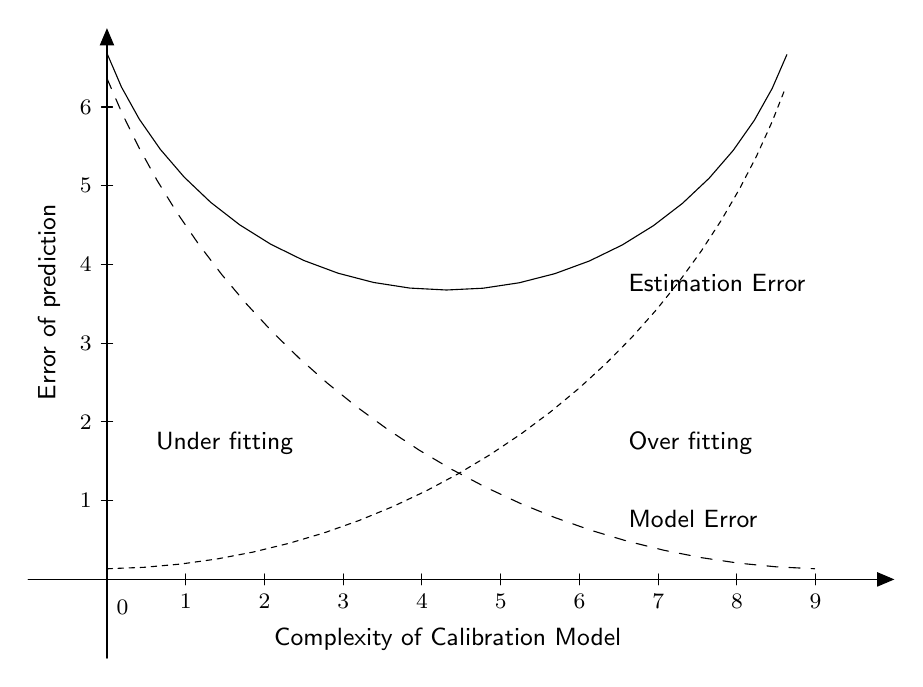
\begin{tikzpicture}[line cap=round,line join=round,>=triangle 45,x=1.0cm,y=1.0cm]
\tikzstyle{every node}=[font=\small\sf]
\draw[->,color=black] (-1.,0.) -- (10.,0.);
\foreach \x in {1,2,3,4,5,6,7,8,9}
\draw[shift={(\x,0)},color=black] (0pt,2pt) -- (0pt,-2pt) node[below] {\footnotesize $\x$};
\draw[->,color=black] (0.,-1.) -- (0.,7.);
\foreach \y in {1,2,3,4,5,6}
\draw[shift={(0,\y)},color=black] (2pt,0pt) -- (-2pt,0pt) node[left] {\footnotesize $\y$};
\draw[color=black] (0pt,-10pt) node[right] {\footnotesize $0$};
\clip(-1.,-1.) rectangle (10.,7.);
\draw [shift={(-0.121669889526,9.43948846317)},dash pattern=on 2pt off 2pt]  plot[domain=4.72546460841:5.93273201445,variable=\t]({1.*9.30535469727*cos(\t r)+0.*9.30535469727*sin(\t r)},{0.*9.30535469727*cos(\t r)+1.*9.30535469727*sin(\t r)});
\draw [shift={(9.23740777921,10.094828387)},dash pattern=on 4pt off 4pt]  plot[domain=3.52560568874:4.68732394366,variable=\t]({1.*9.9630286574*cos(\t r)+0.*9.9630286574*sin(\t r)},{0.*9.9630286574*cos(\t r)+1.*9.9630286574*sin(\t r)});
\draw [shift={(4.3205708351,8.28323005515)}] plot[domain=3.49667738686:5.92421281305,variable=\t]({1.*4.60803364605*cos(\t r)+0.*4.60803364605*sin(\t r)},{0.*4.60803364605*cos(\t r)+1.*4.60803364605*sin(\t r)});
\draw (0.5,2) node[anchor=north west] {$\text{Under fitting}$};
\draw (6.5,2) node[anchor=north west] {$\text{Over fitting}$};
%\draw (-0.00666330535589,0.207513228255) node[anchor=north west] {$\text{Error of Prediction}$};
\draw (-1,5) node[anchor=north west] {$\rotatebox{90.0}{ \text{Error of prediction}  }$};
\draw (6.5,1) node[anchor=north west] {$\text{Model Error}$};
\draw (6.5,4) node[anchor=north west] {$\text{Estimation Error}$};
\draw (2,-0.5) node[anchor=north west] {$\text{Complexity of Calibration Model}$};
\end{tikzpicture}
\caption{Model Error - Estimation Error and Prediction Error}
\label{fig:mdlErrorPlt}
\end{figure}
The relationship between the model complexity and the prediction error is presented in figure-\ref{fig:mdlErrorPlt} with the case of under-fitting and over-fitting of a model.

Furthermore, a model exhibits an \textit{external validity} if it closely predicts the observations that were not used to fit the model parameters (\cite[p.~72]{lattin2003analyzing}). An over-fitted model fails to perform well for those observation that are not included during model parameter estimation. The dataset in this thesis is divided into two parts. The first part includes the observations from Jan 2000 to December 2012 and the second one includes observation onward till November 2014. A cross-validation  approach is utilized on the first set of observation to train the model. The model is used to predict the exchange rate of NOK per Euro from the predictors of the second set of observations. Figure - \ref{fig:calcProcedure} shows the procedure adopted for prediction in this thesis.

\begin{figure}[ht]
\centering
    \includestandalone[width=\linewidth]{include/calcProcedure}
    \caption[Procedure adopted in the thesis]{Procedure adopted in the thesis for model comparison. A cross-validation technique is used to validate the trained dataset. The trained model is used to predict the test response from with prediction errors are obtained.}
    \label{fig:calcProcedure}
\end{figure}

\subsubsection{Cross-Validation}
\label{sssec:crossValidation}
There are various cross-validation techniques among which two are described below;
\begin{description}
\item[ K-Fold Cross-validation:]\hfill \\
The dataset are split into $k$ equal parts. For each $i=1,2,\ldots, k$, a model is fitted leaving out the $i^\text{th}$ portion. A prediction error is calculated for this model. The process is repeated for all $i$. The prediction error for K-fold cross validation is obtained by averaging the prediction error of each of the model fitted.
\item[ Leave-one-out cross validation:]\hfill \\
This is a special case of $k-$ fold cross-validation where $k=n$ (number of observation), i.e, each time one observation is removed and the model is fitted.
\end{description}

\subsubsection{Prediction Error}
\label{sssec:predErr}
Prediction of a model becomes precise if the error is minimum. Models can be compared according to their predictability. Understanding of different measures of prediction error is necessary to acknowledge their predictability and eventually perform model comparison.
\begin{description}
\item[Root Mean Square Error (RMSE)]\hfill\\
RMSE is the measure of how well the model fit the data.
\begin{equation}
\text{RMSE}=\sqrt{\frac{1}{n}\sum_{i=1}^n{\left(y_i-\hat{y}_i\right)^2}}
\end{equation}
Where, \\
$\hat{y}_i$ are predicted values for $y_i$ and\\
$n$ is the number of observation

\item[Root Mean Square Error of Cross-Validation (RMSECV)]\hfill\\
RMSECV gives the models ability to predict new samples that were not present in the model during calibration. It is obtained as,
\begin{align}
\text{RMSECV} &=\sqrt{\frac{\text{PRESS}}{n}} \label{eq:rmsecv}\\
\text{Where, } & \nonumber \\
\text{PRESS} &=\sum_{i=1}^n{\left(y_i-\hat{y}_{(i)}\right)^2} \label{eq:press}
\end{align}
\end{description}
In the special case of leave one out cross validation, $i$ represents each sample.

\subsubsection{R-squared for Prediction}
\label{sssec:rseqPred}
R-squared for prediction is analogs to the R-sq in the case of model estimation. In the case of cross-validation, it is also denoted by $Q^2$. It is obtained by subtracting the ratio of PRESS obtained from equation-\ref{eq:press} to total sum of square from one. i.e,
\begin{equation}
\label{eq:rsqpred}
R^2_{CV}=Q^2=1-\frac{\text{PRESS}}{\text{TSS}} = 1-\frac{\sum_{i=1}^n{\left(y_i-\hat{y}_{(i)}\right)^2}}{\sum_{i=1}^n{\left(y_i-\bar{y}\right)^2}}
\end{equation}
Here, $Q^2<1$ and when prediction is very bad, PRESS may exceed TSS resulting negative value suggesting that the average value is better than the prediction using the model. 

%% Chapter 4 -----------------------------------------------------------------||||

% !Rnw root = ../Main.Rnw

\chapter{Data Analysis}
\label{ch:dataAnalysis}
This chapter will present the analysis report obtained for different models considered in chapter-\ref{chap:modelsmethods}. The analysis process includes following series of steps,

\begin{enumerate}
\item The model is trained from the observation of training period (Jan 2000 - Dec 2012) through cross validation and compare the results
\item Prediction on the average monthly exchange rate of Euro vs Norwegian Krone is made for the test period (Jan 2013 - Nov 2014)
\item Compare them on the basis of criteria discussed in section-\ref{sec:compCriteria}
\end{enumerate}

The summary report of the variables are presented in table (\ref{tbl:sumryTabl}),

{\singlespacing\sffamily

% latex table generated in R 3.1.2 by xtable 1.7-4 package
% Mon Mar 16 07:16:35 2015
\begin{longtable}{rrrrrr}
\caption{Summary Report of all the variables used in this report} \\ 
  \toprule
 \midrule
 & min & median & max & mean & stdev \\ 
  \hline 
\endhead 
\hline 
{\footnotesize Continued on next page} 
\endfoot 
\endlastfoot 
PerEURO & 7.30 & 8.00 & 9.40 & 8.03 & 0.37 \\ 
  KeyIntRate & 1.25 & 2.25 & 7.00 & 3.39 & 2.05 \\ 
  LoanIntRate & 2.25 & 4.00 & 9.00 & 4.87 & 2.32 \\ 
  EuroIntRate & -0.01 & 2.07 & 5.06 & 2.10 & 1.57 \\ 
  CPI & 104.10 & 118.60 & 137.90 & 120.71 & 9.65 \\ 
  OilSpotPrice & 16.70 & 86.29 & 209.29 & 87.64 & 50.80 \\ 
  ImpOldShip & 0.00 & 103.00 & 8099.00 & 229.56 & 641.49 \\ 
  ImpNewShip & 0.00 & 377.00 & 3011.00 & 556.02 & 629.05 \\ 
  ImpOilPlat & 0.00 & 0.00 & 8914.00 & 145.68 & 863.83 \\ 
  ImpExShipOilPlat & 19381.00 & 34812.00 & 51660.00 & 33610.13 & 8437.76 \\ 
  ExpCrdOil & 13125.00 & 22630.00 & 37132.00 & 22771.27 & 4676.88 \\ 
  ExpNatGas & 2457.00 & 11341.00 & 26420.00 & 11883.05 & 6532.83 \\ 
  ExpCond & 0.00 & 751.00 & 2305.00 & 768.94 & 452.03 \\ 
  ExpOldShip & 0.00 & 213.00 & 1948.00 & 342.45 & 358.67 \\ 
  ExpNewShip & 0.00 & 211.00 & 2326.00 & 299.54 & 363.54 \\ 
  ExpOilPlat & 0.00 & 0.00 & 3069.00 & 63.65 & 364.35 \\ 
  ExpExShipOilPlat & 34060.00 & 62457.00 & 90063.00 & 59912.43 & 14947.02 \\ 
  TrBal & 10853.00 & 25001.00 & 48141.00 & 26076.72 & 8257.33 \\ 
  TrBalExShipOilPlat & 11493.00 & 25331.00 & 47250.00 & 26302.36 & 8191.34 \\ 
  TrBalMland & -18150.00 & -9308.00 & -2766.00 & -9120.96 & 3167.78 \\ 
  ly.var & 7.30 & 8.00 & 9.40 & 8.03 & 0.37 \\ 
  l2y.var & 7.30 & 8.00 & 9.40 & 8.03 & 0.37 \\ 
  l.CPI & 103.60 & 118.50 & 137.80 & 120.52 & 9.65 \\ 
   \bottomrule
\label{tbl:sumryTabl}
\end{longtable}


}
%' It is also desirable to see the time series plot of the related variables given in figure -(\ref{fig:timeSeriesPlot})
%' <<timeSeriesPlot, echo=FALSE, fig.cap="Time Series plot of different variables", fig.pos="ht">>=
%' stkTabl<-melt(baseTable[,c("Date", y.var, x.var, y2.var)], id.vars = c("Date", y2.var))
%' plotTS(stkTabl, x.var, y2.var)
%' @

The correlation between response variable and predictor variable helps us to determine their relationship. Figure -(\ref{fig:rpCorPlot}) shows that only few of the predictor variables have significant correlation with response variable. In the figure first and second lagged response variable have strong correlation with response while most of the others have low (weak) correlation. Although, being weak correlation, many of them are statistically significant.
\begin{Schunk}
\begin{figure}

{\centering \includegraphics[width=\maxwidth]{IncluderpCorPlot-1} 

}

\caption[Correlation between response (Exchange Rate) and other predictor variable]{The bars represents the correlation between response variable (\texttt{PerEURO}) and other predictor variable. The bars are shaded with the p-value for their signifance test performed by \texttt{cortest} function. The red horizontal line is the critical value at 5 percent level of significance.\label{fig:rpCorPlot}}
\end{figure}
\end{Schunk}
According to the paper \citetitle{taylor1990interpretation} by \citet{taylor1990interpretation}, the significance of the low correlation, which would have little practical importance, is due to the large number of observation. According to him, a correlation coefficients is an abstract measure which does not give direct precise interpretations. A more useful measure can be obtained during the model fitting.
  %% Common Computation ------------------------------------------------------||||

% !Rnw root = ../Main.Rnw
% Fitting Different Models and saving the results in a list


  %% Multiple Linear Regression with Stepwise reduction -----------------------||||

% !Rnw root = ../Main.Rnw

\section{Multiple Linear Regression}
\label{sec:mlr}
The functional form for determining exchange rate of Norwegian Krone per Euro can be written as,
\begin{align}
\label{eq:mlrFuncForm}
\texttt{PerEURO}&=f(\texttt{interest Rate}, \texttt{Trade}, \texttt{Price}, \texttt{Lag Response})+\texttt{Error} \nonumber \\
&=\alpha_0 +\alpha_1(\texttt{interest Rate})+\alpha_2(\texttt{Trade}) \nonumber \\
&\hspace{1cm}+\alpha_3(\texttt{Price})+\alpha_4(\texttt{Lag Response})+\texttt{Error}
\end{align}
Where, $f$ is a linear function of regression coefficients \bs{\alpha}.

In equation-\ref{eq:mlrFuncForm}, interest Rate include both interest rate of Norway and European Central Bank. Trade incorporates import, export and trade balance of Norway. Similarly, Price include Consumer price index and Oil price. The observation for all the model fitting from this point onward are from the training dataset, i.e. from Jan 2000 to Dec 2012. The detail explanation for the variables are in Appendix A. As described in section - \ref{sec:linRegModel}, the linear model is fitted. The results shows that variables in table-\ref{tbl:lmSumry} has significant effect on the Euro vs Norwegian Krone exchange rate.

{\singlespacing
% latex table generated in R 3.1.2 by xtable 1.7-4 package
% Mon Mar 16 07:16:47 2015
\begin{longtable}{rrr}
\caption{Variables significant at $\alpha=0.05$ while fitting linear model} \\ 
  \hline
 & Estimate & P-value \\ 
  \hline
\texttt{EuroIntRate} & 0.0599 & 0.0307 \\ 
  \texttt{ly.var} & 1.0907 & 0.0000 \\ 
  \texttt{l2y.var} & -0.2358 & 0.0044 \\ 
   \hline
\hline
\label{tbl:lmSumry}
\end{longtable}

}

Since, there are a lot of variables that are not significant at 5\% level of significance in the fitted linear model. So, it is suitable to use variable selection procedure as described in section-\ref{sec:varSelection}.

\section{Variable Selection Procedure}
\label{sec:stepwise}
Variable selection is based on criteria to choose best model form the possible subset. Linear model fitted above when exposed to the those criteria from subsection-\ref{ssec:vsCriteria} for choosing best subset, following results are obtained.

\subsection{Model selection using Mallows $C_p$ and $R^2$ adjusted}
\label{ssec:mcradj}

The best subset is selected using \begin{inlinelist}\item Mallows $C_P$ and \item Adjusted $R^2$ \end{inlinelist}. The number of variable vs these two criteria are plotted in figure-\ref{fig:cpr2plot}. The plot in fig-\ref{fig:cpr2plot1}, shows that including 7 variables, minimize the Mallow's $C_p$ while fig-\ref{fig:cpr2plot2} suggest to include 11 variables including intercept to maximize the adjusted $R^2$.

\begin{Schunk}
\begin{figure}[!ht]

{\centering \subfloat[Mallows Cp vs no. of Variable\label{fig:cpr2plot1}]{\includegraphics[width=0.5\textwidth]{Includecpr2plot-1} }\subfloat[R2 adjusted vs no. of variable\label{fig:cpr2plot2}]{\includegraphics[width=0.5\textwidth]{Includecpr2plot-2} }

}

\caption[Number of variable against the criteria where the red dot corresponds the number of variable to acheave the criteria, i]{Number of variable against the criteria where the red dot corresponds the number of variable to acheave the criteria, i.e. minimum for Cp and maximum for $R^2$ adjusted\label{fig:cpr2plot}}
\end{figure}
\end{Schunk}

The models selected by these criteria when fitted result few insignificant variables. The plot of the t-value in fig-\ref{fig:cpr2mdlplt} has 1 (for $C_p$ criteria) and 6 ($R^2$adj criteria) are insignificant. With fewer variables than the full model, this model has described the variation almost equally as full linear model (table-\ref{tbl:gofSumry}).

\begin{Schunk}
\begin{figure}[!ht]

{\centering \subfloat[Model selected from Mallows' $C_p$ criteria\label{fig:cpr2mdlplt1}]{\includegraphics[width=0.5\textwidth]{Includecpr2mdlplt-1} }\subfloat[Model selected from $R^2$ adjusted criteria\label{fig:cpr2mdlplt2}]{\includegraphics[width=0.5\textwidth]{Includecpr2mdlplt-2} }

}

\caption[Model selected by ]{Model selected by $C_p$ and $R^2$ adjusted criteria. Red and blue bars are significant and insignificant variables respectively. The estimates rounded at 2 decimals are given on top of the bars.\label{fig:cpr2mdlplt}}
\end{figure}
\end{Schunk}

\subsection{Model selection using AIC and BIC criteria}
\label{ssec:aicbicModel}

Applying AIC and BIC criteria to select best model, exhaustive search algorithm as used by \texttt{leaps} package (\cite{lumley2004leaps}) is used in this thesis. Number of variables required to minimize the information criteria is selected as guide by the plot in figure -\ref{fig:aicbicPlot}. For minimum AIC, 11 (fig-\ref{fig:aicbicPlot1}) variables are needed and for minimum BIC, 4(fig-\ref{fig:aicbicPlot2}) are needed to get the best subset model. The models suggested are fitted with results of few insignificant variables (fig-\ref{fig:aicbicmdlplt}). The summary statistic (table-\ref{tbl:gofSumry}) shows that AIC model has larger $R^2$ adjusted than BIC model due to the addition of more variables.

\begin{Schunk}
\begin{figure}[!ht]

{\centering \subfloat[AIC vs no. of Variable\label{fig:aicbicPlot1}]{\includegraphics[width=0.5\textwidth]{IncludeaicbicPlot-1} }\subfloat[BIC vs no. of variable\label{fig:aicbicPlot2}]{\includegraphics[width=0.5\textwidth]{IncludeaicbicPlot-2} }

}

\caption[Number of variable against the AIC vs BIC criteria]{Number of variable against the AIC vs BIC criteria. The red dot corresponds to the number of variables that can minimize the criteria.\label{fig:aicbicPlot}}
\end{figure}
\end{Schunk}
\begin{Schunk}
\begin{figure}[!ht]

{\centering \subfloat[Model selected from minimum AIC criteria\label{fig:aicbicmdlplt1}]{\includegraphics[width=0.5\textwidth]{Includeaicbicmdlplt-1} }\subfloat[Model selected from minimum BIC criteria\label{fig:aicbicmdlplt2}]{\includegraphics[width=0.5\textwidth]{Includeaicbicmdlplt-2} }

}

\caption[Best subset model selected by AIC and BIC criteria]{Best subset model selected by AIC and BIC criteria. Red and blue bars are significant and insignificant variables respectively. The estimates rounded at 2 decimals are given on top of the bars.\label{fig:aicbicmdlplt}}
\end{figure}
\end{Schunk}


\subsection{Step wise procedures based on F-value}
\label{ssec:stepwisePvalue}
The models fitted in previous sub sections resulted with some insignificant variables because the criteria there was based on model statistics other than the p-value of the respective variables. The step wise procedure based on the F-test fit the model removing the insignificant variable one at a time in backward search and adding variable one at a time in forward search. The fitted results (fig-\ref{fig:FbasedModelSubset}) for the models fitted with forward (fig-\ref{fig:FbasedModelSubset1}) and backward (fig-\ref{fig:FbasedModelSubset2}) step wise procedure show that all the variables are significant at 5 percent except (\texttt{ExpCrdOil}) in backward model since the \texttt{alpha-to-remove} and \texttt{alpha-to-enter} criteria for the process are set at 0.1.

\begin{Schunk}
\begin{figure}[!ht]

{\centering \subfloat[Model selected from stepwise forward selection prcedure\label{fig:FbasedModelSubset1}]{\includegraphics[width=0.5\textwidth]{IncludeFbasedModelSubset-1} }\subfloat[Model selected from stepwise backward elimination procedure\label{fig:FbasedModelSubset2}]{\includegraphics[width=0.5\textwidth]{IncludeFbasedModelSubset-2} }

}

\caption[Best subset model selected by F-test based criteria]{Best subset model selected by F-test based criteria. Red and blue bars are significant and insignificant variables respectively. The estimates rounded at 2 decimals are given on top of the bars.\label{fig:FbasedModelSubset}}
\end{figure}
\end{Schunk}

\begin{Schunk}
\begin{figure}[!htb]

{\centering \includegraphics[width=\maxwidth]{IncludevifPlot-1} 

}

\caption[Variance Inflation Factor (VIF) of different models]{Variance Inflation Factor (VIF) of different models. The red bars represents the variables with VIF greater than 10.\label{fig:vifPlot}}
\end{figure}
\end{Schunk}

Here, the models suggested by $R^2$ criteria and AIC are same. Similar BIC and step wise forward selection based on F-test also have suggested the same model. In addition, models fitted with minimum Cp criteria and F-test based backward elimination procedure results with similar set of variables. Despite of explaining enough variation in response, some of these models have severe multicollinearity problem (Fig-\ref{fig:vifPlot}) since the VIF (Variance Inflation Factor) of some of the variables included in the model are much larger than 10 which is usually considered as rule of thumb (\cite{OabRob2007}) for measuring multicollinearity.

Multicollinearity in a model distorts the estimate and consequently distorts the prediction made by the model. An alternative solution for the multicollinearity problem is using principal component related model such as PLS and PCR or one can use ridge regression as well. 
  
  %% Principal Component Analysis and Regression ------------------------------||||

% !Rnw root = ../Main.Rnw
\section{Principal Component Analysis}
\label{sec:pcaAnalysis}

Principal Component Analysis(PCA) creates a new set of mutually orthogonal and uncorrelated variables called components. The PCA analysis is done from full dataset (Jan 2000 - Nov 2014) which are first centered and scaled.

Since the standard deviation of first 6 principal components are greater than one (table-\ref{tbl:pcaSumry}), they are explaining the variation greater than the original variables. In addition around 99 percent of variation in x-variables are explained by 13 components of PCA which is seen on the cumulative proportion of variation in the same table.

{\singlespacing\sffamily
% latex table generated in R 3.1.2 by xtable 1.7-4 package
% Mon Mar 16 07:16:50 2015
{\footnotesize
\begin{longtable}{rrrr|rrrr}
\caption{Dispersion of data explained by principal components} \\ 
  \hline
\hline
Comp & Std.Dev & Var.Prop & Cum.Var.Prop & Comp & Std.Dev & Var.Prop & Cum.Var.Prop \\ 
  \hline 
\endhead 
\hline 
{\scriptsize Continued on next page} 
\endfoot 
\endlastfoot 
   1 & 3.018 & 0.414 & 0.414 &    8 & 0.958 & 0.042 & 0.867 \\ 
     2 & 1.602 & 0.117 & 0.531 &    9 & 0.891 & 0.036 & 0.903 \\ 
     3 & 1.376 & 0.086 & 0.617 &   10 & 0.848 & 0.033 & 0.936 \\ 
     4 & 1.216 & 0.067 & 0.684 &   11 & 0.787 & 0.028 & 0.964 \\ 
     5 & 1.054 & 0.051 & 0.734 &   12 & 0.620 & 0.017 & 0.981 \\ 
     6 & 1.023 & 0.048 & 0.782 &   13 & 0.446 & 0.009 & 0.990 \\ 
     7 & 0.978 & 0.044 & 0.825 &   14 & 0.274 & 0.003 & 0.994 \\ 
   \hline
\hline
\label{tbl:pcaSumry}
\end{longtable}
}

}

\section{Principal Component Regression}
\label{sec:pcrAnalysis}

A prediction model based on the few components instead of all original variables, considered in PCA, not only remove the complexity of the model but also gives mutually orthogonal and uncorrelated components (new variables) which removes the multicollinearity problem during model fitting. A PCA model is fitted with observations in the training dataset (Jan 2000 - Dec 2012), the variation explained on both \mbf{X} and \mbf{Y} are presented in table-\ref{tbl:pcrSumry}.

The results shows that the first 6 components which have explained larger variance than the actual variable, as seen in PCA, explain about 84 percent of variation in response. If 16 components are considered, the percentage of explained variation in response rises to almost 90 percent.

{\singlespacing\sffamily
% latex table generated in R 3.1.2 by xtable 1.7-4 package
% Mon Mar 16 07:16:50 2015
{\footnotesize
\begin{longtable}{rrr|rrr|rrr}
\caption{Percentage of variation explained by PCR model in response and predictor} \\ 
  \hline
Comp & X & PerEURO & Comp & X & PerEURO & Comp & X & PerEURO \\ 
  \hline
  1 & 41.05 & 0.52 &   8 & 86.58 & 85.56 &  15 & 99.61 & 89.72 \\ 
    2 & 53.14 & 43.73 &   9 & 90.19 & 85.62 &  16 & 99.86 & 91.80 \\ 
    3 & 61.61 & 77.57 &  10 & 93.42 & 85.63 &  17 & 99.98 & 91.80 \\ 
    4 & 68.22 & 79.93 &  11 & 96.27 & 85.82 &  18 & 99.99 & 91.80 \\ 
    5 & 73.31 & 84.14 &  12 & 98.02 & 86.67 &  19 & 100.00 & 91.82 \\ 
    6 & 78.05 & 84.14 &  13 & 99.02 & 86.82 &  20 & 100.00 & 91.86 \\ 
    7 & 82.50 & 84.31 &  14 & 99.35 & 86.87 &  21 & 100.00 & 91.88 \\ 
   \hline
\hline
\label{tbl:pcrSumry}
\end{longtable}
}

}
  
  %% Partial Least Square Regression ------------------------------------------||||

% !Rnw root = ../Main.Rnw
\section{Partial Least Square Regression}
\label{sec:plsAnalysis}

Principal Component Regression aims to collect the variation present in predictor variables with its first few components but it does not give any consideration to the variation present in response. In many cases, PCA can capture the variation present in response variable but in other situations, it fails or become slower (need more components) to explain it. In such case, Partial Least Square (PLS) regression can be a solution.

Partial Least Square (PLS) regression when fitted with six components can explain more than 91 percent of variation in Exchange Rate while it explain only 73 percent of variation in predictor variables. Table-\ref{tab:plsSumry} shows that the percentage of variation explained in Exchange rate has increased dramatically in first two components which then settled down. If all the components are considered in the model, the variation explained in the case resembles with the $R^2$ value of linear model. Since, the later components contains only residuals and have no useful information, the idea of including them only increases the model complexity and can leads to over-fitting which is also true for PCR model.

{\singlespacing\sffamily
% latex table generated in R 3.1.2 by xtable 1.7-4 package
% Mon Mar 16 07:16:50 2015
{\footnotesize
\begin{longtable}{rrr|rrr|rrr}
\caption{Percentage of variation Explained by PLS model in Response and Predictor} \\ 
  \hline
Comp & X & PerEURO & Comp & X & PerEURO & Comp & X & PerEURO \\ 
  \hline
  1 & 13.63 & 77.96 &   8 & 79.16 & 91.75 &  15 & 95.34 & 91.81 \\ 
    2 & 50.59 & 83.70 &   9 & 81.66 & 91.79 &  16 & 99.64 & 91.81 \\ 
    3 & 60.46 & 86.75 &  10 & 83.62 & 91.80 &  17 & 99.87 & 91.82 \\ 
    4 & 65.73 & 87.90 &  11 & 87.41 & 91.80 &  18 & 99.99 & 91.82 \\ 
    5 & 68.68 & 89.53 &  12 & 89.23 & 91.80 &  19 & 100.00 & 91.82 \\ 
    6 & 72.80 & 90.62 &  13 & 91.53 & 91.80 &  20 & 100.00 & 91.88 \\ 
    7 & 75.70 & 91.54 &  14 & 94.48 & 91.80 &  21 & 100.00 & 91.90 \\ 
   \hline
\hline
\label{tab:plsSumry}
\end{longtable}
}

}


\begin{Schunk}
\begin{figure}[!htpb]

{\centering \includegraphics[width=\maxwidth]{IncludePLSnPCRcompPlot-1} 

}

\caption[Variation Explained by PLS and PCR]{Variation Explained by PLS and PCR model on Predictor Variable and Response Variable\label{fig:PLSnPCRcompPlot}}
\end{figure}
\end{Schunk}
The actual difference between PLS and PCR model can also be observed from the variation explained plot in figure-\ref{fig:PLSnPCRcompPlot}. The plot shows that PCR explain more of the predictor variation with few components while PLS explain more of the response variation with fewer components than PCR. However, on taking more components, both the models agrees at some point.

\section{Ridge Regression}
\label{sec:ridgeReg}

Ridge regression in this thesis is performed using \texttt{ridge} package. Although the package has implement semi-automatic method (\cite{cule2012semi}) to choose the ridge regression parameter($\lambda$), this thesis has chosen $\lambda$ from a range [0, 0.01] by implementing cross validation technique. The parameter is found to be 0.005 which can results minimum RMSECV. An alternative way is to choose $\lambda$ by maximizing the $R^2$ predicted (fig-\ref{fig:lmdaTuning}). The parameter is also known as shrinkage parameter as it shrink the coefficients estimates which was enlarged by the Multicollinearity problem. Coefficient estimates plotted in figure -\ref{fig:coefPlot} shows that the coefficients obtained from linear model has fluctuated due to the presence of multicollinearity. In the figure, the coefficients obtained from ridge regression were pulled down towards zero.


\begin{Schunk}
\begin{figure}[htbp]

{\centering \includegraphics[width=\maxwidth]{IncludelmdaTuning-1} 

}

\caption[RMSE and R2pred plots for different ridge regression paramter ]{RMSE and R2pred plots for different ridge regression paramter $\lambda$. The red dots refers to the maximum $R^2$ pred and minimum RMSEP.\label{fig:lmdaTuning}}
\end{figure}
\end{Schunk}
  
  %% Partial Least Square Regression ------------------------------------------||||

% !Rnw root = ../Main.Rnw
\section{Cross Validation}
\label{sec:crossvalidation}




Usually, a predictive model is expected to predict test responses not included in the sample. A model which can well predict the in-sampled observation may not perform well for out-of-sample observations. Cross-validation can verify the ability of model during prediction in such cases. Since time-series has a sequential form of ordered by date, a random prediction is unsuitable. A cross-validation technique is applied to the training dataset dividing them into 12 consecutive segments. Each time a segment is removed from the fitted model which then predict the segment which was not included. The process is repeated for all the segments and RMSECV and $R^2$ prediction ($Q^2$) are computed using the equation-\ref{eq:rmsecv} and equation-\ref{eq:rsqpred} respectively. The validation is performed for all the models discussed above, from which RMSECV and $R^2$ predicted are computed as in table-\ref{tbl:valdSumry}.

The table shows that PLS with 8 components and PCR with 16 components have least RMSECV and highest $R^2$ predicted. This also indicate that those models speaks better with the new observation, that are not included in the models, in compared with other linear models.

\begin{Schunk}
\begin{figure}[htpb]

{\centering \includegraphics[width=\maxwidth]{IncludermsepPlot-1} 

}

\caption[RMSEP plot for PCR and PLS]{RMSEP plot for PCR and PLS model with and without cross-validation. Cross-validation is done with 12 observation in each consecutive segments within training dataset.\label{fig:rmsepPlot}}
\end{figure}
\end{Schunk}

Further analysis is made on PLS and PCR models by computing the RMSECV and $R^2$ predicted, and plotted them against all the components. Figure-\ref{fig:rmsepPlot} shows that the curve of RMSECV and $R^2$ predicted fluctuate over components in contrast to the results without cross-validation. In the case without cross-validation, RMSEP continually decreases initially and gets stable and $R^2$ predicted continually increases and gets stable. 

In the plot, PLS model starts predicting better from very beginning while PCR meets the quality only after considering 16 components. From the results of cross-validation, it is expected to have best prediction from the PLS model with 8 components.

\section{Prediction on test Data}
\label{sec:predTest}


After getting some idea about the prediction ability of a model from cross-validation procedure, it is time to observe its performance in the case of test dataset. Exchange Rate from Jan 2013 to Nov 2014 are predicted using the training dataset which includes the financial and commodity variables from Jan 2000 to Dec 2012. For the prediction, a multiple linear regression model, its subsets selected from various selection criteria, a PLS model with 6, 7, 8, 9 components, a PCR model with 15, 16, 17 components and a ridge regression model with parameter $\lambda=0.005$ are applied. A prediction is also made on the calibration set and the results for both predictions - Training set and Test set are plotted on figure-\ref{fig:forecast}.

The plot shows that the predictions from all the models are very close to the true value. From the RMSEP and R2pred value at the top left corner of each panel, PLS model with 7 components have predicted the test observations more closely as they have minimum RMSEP and maximum $R^2$pred. However, in the case of in-sample prediction on the training dataset, linear model has least RMSEP and maximum $R^2$pred, but since it is suffered from multicollinearity problem, PLS model with 9 components and PCR with 17 components can be an alternative.

\section{Comparison of Models}
\label{sec:modelComp}

Models can be compared on the basis of their predictability and goodness of fit. As discussed in chapter-\ref{chap:modelsmethods}, the goodness of fit of a model can be accessed from \begin{inlinelist} \item variation the model has described,\item distribution of residuals and \item information criteria  \end{inlinelist}. Also, the predictability of the model can be compared from \begin{inlinelist} \item RMSEP and \item $R^2$ predicted \end{inlinelist} for calibration and test dataset.

\subsection{Goodness of fit}
\label{ssec:gof}
All the linear models (full and subset) have explained almost 90 percent of variation in response which is seen in $R^2$ and $R^2$ adjusted presented in table-\ref{tbl:gofSumry}. Further, the models are significant since their p-value is very close to zero. Comparing the models, \texttt{cp.model} and \texttt{backward} have smallest AIC value while \texttt{bicMdl} and \texttt{forward} models have smallest BIC. Each pair of these models have selected the same set of variables each set can be considered as equivalent. In addition, \texttt{r2.model} and \texttt{aicMdl} models have maximum $R^2$adj and minimum residual standard error (sigma).
% latex table generated in R 3.1.2 by xtable 1.7-4 package
% Mon Mar 16 07:17:03 2015
\begin{table}[ht]
\centering
\caption{Summary statistic and information criteria for model comparison} 
\label{tbl:gofSumry}
\begin{tabularx}{\textwidth}{Xrrrrrrr}
  \hline
Model & AIC & BIC & R.Sq & R.Sq.Adj & Sigma & F.value & P.value \\ 
  \hline
linear & -207.1781 & -133.9816 & 0.9190 & 0.9056 & 0.1157 & 68.5936 & 0.0000 \\ 
  cp.model & -230.3234 & -205.9245 & 0.9143 & 0.9108 & 0.1124 & 264.8486 & 0.0000 \\ 
  r2.model & -227.9952 & -191.3969 & 0.9173 & 0.9116 & 0.1119 & 160.9059 & 0.0000 \\ 
  aicMdl & -227.9952 & -191.3969 & 0.9173 & 0.9116 & 0.1119 & 160.9059 & 0.0000 \\ 
  bicMdl & -229.2344 & -213.9852 & 0.9103 & 0.9085 & 0.1139 & 514.1058 & 0.0000 \\ 
  forward & -229.2344 & -213.9852 & 0.9103 & 0.9085 & 0.1139 & 514.1058 & 0.0000 \\ 
  backward & -230.3234 & -205.9245 & 0.9143 & 0.9108 & 0.1124 & 264.8486 & 0.0000 \\ 
   \hline
\end{tabularx}
\end{table}


Since prediction is the objective, \texttt{r2.model} and \texttt{aicMdl} model can be considered as better than other linear models since they have smallest residual standard error and explain the response variable better than others. Further, the residues obtained from this selected set of regression models are nearly Normal and random which can be seen from the diagnostic plots in appendix-\ref{diagPlot} but still there are some outliers due to the global financial crisis discussed in section-\ref{sec:crisisEffect}. Despite having outliers in these models, the outliers are not very influential as their cook's distance is still less than a unity.

In the case of PLS and PCR models, the residues obtained from them after considering 7 for PLS and 17 for PCR are plotted in appendix-\ref{fig:residPlot} are also random. This shows that the models have not missed important information and the models does not have any effect of autocorrelation anymore.

\subsection{Predictability}
\label{ssec:prdblty}
The main concert of this thesis is about the predictability of a model. The predictability of a model is measured using RMSEP and $R^2$ predicted. A model exhibit different nature in the case of prediction in training dataset, during cross-validation and when implementing it to predict the test dataset. The plot in fig-\ref{fig:ValdSumryPlot} shows this discrepancies.


\begin{Schunk}
\begin{figure}

{\centering \includegraphics[width=\maxwidth]{IncludeValdSumryPlot-1} 

}

\caption[Comparision of Model on the ground of calibration model, cross-validation models and prediction model on the basis of RMSEP and ]{Comparision of Model on the ground of calibration model, cross-validation models and prediction model on the basis of RMSEP and $R^2$ predicted\label{fig:ValdSumryPlot}}
\end{figure}
\end{Schunk}



From all the candidate models considered as best, RMSEP and $R^2$ predicted are tabulated for training dataset, during cross-validation and for test dataset. It is observed that Linear Model has generated least prediction error and maximum $R^2$pred when predicting the samples on training dataset. During cross-validation, PLS model with 8 components perform best by giving least RMSEP (0.123). The main concert of this thesis is the prediction of test dataset. PLS model with 7 components producing RMSEP (0.1008) and $R^2$pred (0.108) can be considered as the best model.
% latex table generated in R 3.1.2 by xtable 1.7-4 package
% Mon Mar 16 07:17:04 2015
\begin{table}[ht]
\centering
\caption{Validation result containing RMSEP and R2pred for training set, cross-validation set and test set} 
\label{tbl:valdSumry}
\begin{tabular}{rrrrrrr}
  \hline Model & 
                 \multicolumn{2}{c}{Training} & 
                 \multicolumn{2}{c}{Cross Validation} & 
                 \multicolumn{2}{c}{Test} \\ 
                 \cline{2-7} & RMSEP & R2pred & RMSEP & R2pred & RMSEP & R2pred \\ \hline
  \hline
Linear & 0.1068 & 0.9190 & 0.1445 & 0.8229 & 0.1111 & 0.8961 \\ 
  AICModel & 0.1079 & 0.9173 & 0.1410 & 0.8308 & 0.1068 & 0.9040 \\ 
  BICModel & 0.1124 & 0.9103 & 0.1278 & 0.8631 & 0.1027 & 0.9112 \\ 
  BackModel & 0.1099 & 0.9143 & 0.1468 & 0.8181 & 0.1188 & 0.8812 \\ 
  Ridge & 0.1076 & 0.9177 & 0.1352 & 0.8408 & 0.1083 & 0.9012 \\ 
  PCR.Comp15 & 0.1203 & 0.8972 & 0.1343 & 0.8730 & 0.1254 & 0.8677 \\ 
  PCR.Comp16 & 0.1075 & 0.9180 & 0.1221 & 0.8928 & 0.1048 & 0.9075 \\ 
  PCR.Comp17 & 0.1075 & 0.9180 & 0.1236 & 0.8901 & 0.1048 & 0.9076 \\ 
  PLS.Comp6 & 0.1150 & 0.9062 & 0.1316 & 0.8755 & 0.1080 & 0.9018 \\ 
  PLS.Comp7 & 0.1092 & 0.9154 & 0.1263 & 0.8847 & 0.1008 & 0.9144 \\ 
  PLS.Comp8 & 0.1078 & 0.9175 & 0.1225 & 0.8922 & 0.1058 & 0.9057 \\ 
  PLS.Comp9 & 0.1075 & 0.9179 & 0.1226 & 0.8920 & 0.1051 & 0.9069 \\ 
   \hline
\end{tabular}
\end{table}


\section{Coefficients Estimates}
\label{sec:coefEst}

\begin{Schunk}
\begin{figure}[htpb]

{\centering \includegraphics[width=\maxwidth]{IncludecoefPlot-1} 

}

\caption[Cofficients estimates for predictor variables]{Comparision plot for coefficients estimates of predictor variables. The variables are sorted according to their estimates from linear model.\label{fig:coefPlot}}
\end{figure}
\end{Schunk}
The estimated coefficients of a linear model are larger in magnitude than the Ridge, PCR and PLS models. The first lagged response has very high (1.0907) positive coefficient and has large influence on the model. The plot in figure-\ref{fig:coefPlot} shows that Import of old ship has larger coefficients than other import and export variables. On Dec 2008, a large sum of money is used to import elderly ships in Norway (fig-\ref{fig:tsPlotImp}) which has an impact on its effect on the exchange rate models.

In addition, the PLS (8 Comp) and PCR (16 Comp) model have identified Oil spot price, Key interest rate, CPI and its lagged value as influential variable apart from the two lagged response variables. Some of the variables having higher coefficients obtained from these two models are presented in table -\ref{tbl:coefEstdTbl}.

{\singlespacing\scriptsize
% latex table generated in R 3.1.2 by xtable 1.7-4 package
% Mon Mar 16 07:17:04 2015
\begin{table}[ht]
\centering
\caption[Coefficient Estimate for PLS and PCR model]{Top three (both positive and negative) Coefficient Estimate of PLS and PCR model} 
\label{tbl:coefEstdTbl}
\begin{tabular}{rrrrrrr}
  \hline
 & l2y.var & LoanIntRate & KeyIntRate & ly.var & EuroIntRate & ImpOldShip \\ 
  \hline
pcr & -0.0863 & -0.0328 & -0.0317 & 0.4081 & 0.0902 & 0.0464 \\ 
  pls & -0.0801 & -0.0337 & -0.0280 & 0.4044 & 0.0918 & 0.0476 \\ 
   \hline
\end{tabular}
\end{table}

}

\section{Autocorrelation and its resolution}
\label{sec:autocorr}
Due to autocorrelation the lagged response variable are included in the model. Since the partial autocorrelation function (PACF) plot of the residuals in appendix-\ref{fig:pacfPlot} shows that the error terms are free from autocorrelation. This justify the inclusion of the lagged variable in the model to remove autocorrelation present.
 
%% Chapter 5 -----------------------------------------------------------------||||

% !Rnw root = ../Main.Rnw

\chapter{Discussions and Conclusion}
\label{ch:DiscsConclusion}

\section{Some discussions}
\label{sec:discussions}
It is always a preliminary idea to use basic liner model. A linear model with full set of variables does not always results on selecting important and significant variables. This thesis has build both linear models and component regression (PCR and PLS). From the first group, linear models and their subset were compared on the basis of Mallows Cp, AIC, BIC and $R^2$adj criteria. Here prediction is the interest, the subset models with maximum $R^2$adj and minimum Residual sum of square is preferred, i.e. \texttt{aicMdl}. A diagnostic plot for the model in appendix - \ref{fig:diagPlot} contains four plots. 

The first one in the plot is the fitted value vs square root of standardize residuals. In the plot the crisis period have higher fitted values and have greater residues. the second plot elaborate the problem a step forward. The plot clearly shows that the distortion on the normality are due the observation of the crisis period. The third plot of cook's distance shows the most of the outlier observation are from the crisis period which have larger influence. Their influence is shown in the fourth plot of Leverage vs standardized residuals.

Although have some influential outliers, the observations are still within the limit. The value of most influencing outlier is from Dec 2008 which is a crucial time point of the recent great recession (\cite{FinCrisis2009Kred}).

The loading plot (appendix-\ref{fig:loadingPlot}) for PLS model shows that component one constitute the effect of lagged value of response which generate high positive values in loading of first components. Some of the export related variables, which has positive contribution on second components, has negative contribution on first components. The second components has high negative influence of interest rate variable while this component has positive contribution of the oil spot price. Since there is more than 77 percent of contribution of first component, it shows that the lagged value of response has huge contribution on explaining the variation present on Exchange rate. In addition, the effect of interest rate , Oil price and export related variables are gathered by the second components.

Additionally, score plots (appendix-\ref{fig:scorePlot}) for the first three components of partial least square regression revels the fact that the second components which contains 36.96 percent of \mbf{X} variation has accumulated the effect of crisis period. Most of the positive large scores of second components are from the crisis period.

Although \texttt{aicMdl} model is considered better than other linear models from the criteria of goodness of fit, it still lag behind PLS and PCR models on RMSEP and $R^2$pred for cross-validation and test data prediction. Figure-\ref{fig:ValdSumryPlot} shows that the linear model has predict the in-sample observations closer than other models but for out-of-sample observations, PCR and PLS models has out performed the linear models.

\section{Conclusions}
\label{sec:conclusion}
\begin{enumerate}
\item From this study, it is found that future value of Exchange rate of NOK per Euro depends on its past values very much. Apart from the past values of exchange rate, the commodity and financial variables especially interest rate of Euro zone, loan interest rate, import of old ships, first lag of CPI have contributed for explaining the variation present in exchange rate.
\item Forecasting of time-series data usually suffers with autocorrelation and multicollinearity problems. An autoregressive model alleviate the problem of autocorrelation in many situations. This also has become true for this study since the residues obtained from the fitted model with lagged dependent variable does not contain any autocorrelations. Although some of the linear models contains multicollinearity, by the use of principal components and latent variables, the problem was resolved.
\item Forecasting exchange rate is often desired rather than its past prediction. Among the various models fitted in this dissertation, partial least square regression with just seven components has outperformed other models while predicting exchange rate of January 2013 to November 2014. Since, the model has settled down the problems of multicollinearity and autocorrelation and performed fine predictions, the use of latent variable model in the case of time series forecasting is a better alternative.
\end{enumerate}

\section{Further Study}
\label{sec:furtherStudy}
Since this dissertation has included data of trade balance, interest rate and consumer price index, an extensive study should be performed by including more relevant variables for deeper understanding of exchange rate dynamics. A study on exchange rate other than NOK vs Euro is recommended for cross examination and validation of the model this thesis has prescribed. In addition, a comparison of the latent variable models with contemporary models that economist are practicing is also suggested.

%% Reference ----------------------------------------------------------------- |||
% Make the bibliography single spaced
\singlespacing
\printbibliography

% add the Bibliography to the Table of Contents
\cleardoublepage
\ifdefined\phantomsection
  \phantomsection  % makes hyperref recognize this section properly for pdf link
\else
\fi
\addcontentsline{toc}{chapter}{Bibliography}

\appendix
  %% Data Description ------------------------------||||

% !Rnw root = ../Main.Rnw

\chapter{Data Description}
\label{ch:dataDesc}

The variables used in this paper are listed in following table along with the code used for them.
% latex table generated in R 3.1.2 by xtable 1.7-4 package
% Mon Mar 16 07:17:06 2015
\begin{tabularx}{\textwidth}{lX}
  \toprule
Code & Description \\ 
  \hline \endhead  \midrule
\texttt{Date} & Date \\ 
  \texttt{PerEURO} & Exchange Rate of NOK per Euro \\ 
  \texttt{PerUSD} & Exchange Rate of NOK per USD \\ 
  \texttt{KeyIntRate} & Key policy rate (Percent) \\ 
  \texttt{LoanIntRate} & Overnight Lending Rate (Nominal) \\ 
  \texttt{EuroIntRate} & Money market interest rates of Euro area (EA11-2000, EA12-2006, EA13-2007, EA15-2008, EA16-2010, EA17-2013, EA18) \\ 
  \texttt{CPI} & Consumer Price Index (1998=100) \\ 
  \texttt{OilSpotPrice} & Europe Brent Spot Price FOB (NOK per Barrel) \\ 
  \texttt{ImpOldShip} & Imports of elderly ships (NOK million) \\ 
  \texttt{ImpNewShip} & Imports of new ships (NOK million) \\ 
  \texttt{ImpOilPlat} & Imports of oil platforms (NOK million) \\ 
  \texttt{ImpExShipOilPlat} & Imports excl. ships and oil platforms (NOK million) \\ 
  \texttt{ExpCrdOil} & Exports of crude oil (NOK million) \\ 
  \texttt{ExpNatGas} & Exports of natural gas (NOK million) \\ 
  \texttt{ExpCond} & Exports of condensates (NOK million) \\ 
  \texttt{ExpOldShip} & Exports of elderly ships (NOK million) \\ 
  \texttt{ExpNewShip} & Exports of new ships (NOK million) \\ 
  \texttt{ExpOilPlat} & Exports of oil platforms (NOK million) \\ 
  \texttt{ExpExShipOilPlat} & Exports excl. ships and oil platforms (NOK million) \\ 
  \texttt{TrBal} & Trade balance (Total exports - total imports) (NOK million) \\ 
  \texttt{TrBalExShipOilPlat} & Trade balance (Exports - imports, both excl. ships and oil platforms) (NOK million) \\ 
  \texttt{TrBalMland} & Trade balance (Mainland exports - imports excl. ships and oil platforms) (NOK million) \\ 
  \texttt{ly.var} & First Lag Exchange Rate of NOK per Euro \\ 
  \texttt{l2y.var} & Second Lag Exchange Rate of NOK per Euro \\ 
  \texttt{l.CPI} & First Lag of Consumer Price Index \\ 
  \texttt{ExcChange} & Change status of Exchange Rate (Increase, Decrease and Unchange) \\ 
  \texttt{Testrain} & Test and Train seperation of data \\ 
  \texttt{season} & Seasons \\ 
   \bottomrule
\end{tabularx}



  

% !Rnw root = ../Main.Rnw

\chapter{R packages used}
\label{ch:rpkgsUsed}



% latex table generated in R 3.1.2 by xtable 1.7-4 package
% Mon Mar 16 07:17:06 2015
\begin{tabularx}{\textwidth}{lrX}
  \toprule
Name & Version & Title \\ 
  \hline \endhead  \midrule
\texttt{MASS}(\cite{MASS2001WNV}) & 7.3-35 & Support Functions and Datasets for Venables and Ripley's MASS \\ 
  \texttt{car}(\cite{car2011FJnWS}) & 2.0-22 & Companion to Applied Regression \\ 
  \texttt{pls}(\cite{pls2013MBH}) & 2.4-3 & Partial Least Squares and Principal Component regression \\ 
  \texttt{xtable}(\cite{xtable2014DD}) & 1.7-4 & Export tables to LaTeX or HTML \\ 
  \texttt{grid}(\cite{gridExtra2012AB}) & 3.1.2 & The Grid Graphics Package \\ 
  \texttt{gridExtra}(\cite{gridExtra2012AB}) & 0.9.1 & functions in Grid graphics \\ 
  \texttt{knitr}(\cite{knitr2013XY}) & 1.8 & A General-Purpose Package for Dynamic Report Generation in R \\ 
  \texttt{leaps}(\cite{leaps2009LT}) & 2.9 & regression subset selection \\ 
  \texttt{zoo}(\cite{zoo2005ZAGG}) & 1.7-11 & S3 Infrastructure for Regular and Irregular Time Series (Z's
ordered observations) \\ 
  \texttt{gdata}(\cite{gdata2014WG}) & 2.13.3 & Various R programming tools for data manipulation \\ 
  \texttt{ridge}(\cite{ridge2014CE}) & 2.1-3 & Ridge Regression with automatic selection of the penalty
parameter \\ 
  \texttt{plyr}(\cite{plyr2011WH}) & 1.8.1 & Tools for splitting, applying and combining data \\ 
  \texttt{dplyr}(\cite{dplyr2014WHFR}) & 0.3.0.2 & A Grammar of Data Manipulation \\ 
  \texttt{ggplot2}(\cite{ggplot22009WH}) & 1.0.0 & An implementation of the Grammar of Graphics \\ 
  \texttt{reshape2}(\cite{reshape22007WH}) & 1.4 & Flexibly reshape data: a reboot of the reshape package. \\ 
  \texttt{scales}(\cite{scales:2014Wickham}) & 0.2.4 & Scale functions for graphics. \\ 
  \texttt{mixlm}(\cite{mixlm2014SK}) & 1.0.7 & Mixed Model ANOVA and Statistics for Education \\ 
  \texttt{graphics}(\cite{R2014Rcore}) & 3.1.2 & The R Graphics Package \\ 
  \texttt{grDevices}(\cite{R2014Rcore}) & 3.1.2 & The R Graphics Devices and Support for Colours and Fonts \\ 
  \texttt{utils}(\cite{R2014Rcore}) & 3.1.2 & The R Utils Package \\ 
  \texttt{datasets}(\cite{R2014Rcore}) & 3.1.2 & The R Datasets Package \\ 
  \texttt{methods}(\cite{R2014Rcore}) & 3.1.2 & Formal Methods and Classes \\ 
  \texttt{base}(\cite{R2014Rcore}) & 3.1.2 & The R Base Package \\ 
   \bottomrule
\end{tabularx}


  

% !Rnw root = ../Main.Rnw

\chapter{Some Relevent Plots}
\label{ch:revPlots}
\begin{Schunk}
\begin{figure}[h!]

{\centering \includegraphics[width=\maxwidth]{IncludediagPlot-1} 

}

\caption[Diagnostic plot for the subset of linear model selected from minimum ]{Diagnostic plot for the subset of linear model selected from minimum $C_p$ criteria. The red bubble represents the two years of crisis period from june 2007 till june 2009. The size of a bubbles in the plot of leverage vs standardized residuals on bottom right corner represents the cooks' distance.\label{fig:diagPlot}}
\end{figure}
\end{Schunk}

\begin{Schunk}
\begin{figure}[!h]

{\centering \includegraphics[width=\maxwidth]{IncludeloadingPlot-1} 

}

\caption[Scatter loading plot of PLS with its first and second components]{Scatter loading plot of PLS with its first and second components. Labels are colored according to their domain of fields.\label{fig:loadingPlot}}
\end{figure}
\end{Schunk}

\begin{Schunk}
\begin{figure}[!h]

{\centering \includegraphics[width=\maxwidth]{IncludescorePlot-1} 

}

\caption[Scoreplot of first three component of PLS regression]{Scoreplot of first three component of PLS regression. The red bubbles represents the crisis period.\label{fig:scorePlot}}
\end{figure}
\end{Schunk}

\begin{Schunk}
\begin{figure}

{\centering \includegraphics[width=\maxwidth]{IncluderesidPlot-1} 

}

\caption[Residuals obtained after fitting the model]{Residuals obtained after fitting the model. The plot exhibit randomness without any kind of pattern.\label{fig:residPlot}}
\end{figure}
\end{Schunk}

\begin{Schunk}
\begin{figure}

{\centering \includegraphics[width=\maxwidth]{IncludepacfPlot-1} 

}

\caption[Partial Autocorrelation Function (PACF) of Residuals obtained after fitting the model]{Partial Autocorrelation Function (PACF) of Residuals obtained after fitting the model. The plot exhibit randomness without any kind of pattern.\label{fig:pacfPlot}}
\end{figure}
\end{Schunk}

\begin{Schunk}
\begin{figure}

{\centering \includegraphics[width=\maxwidth]{Includeforecast-1} 

}

\caption[Prediction made on trained and test dataset using different models]{Prediction made on trained and test dataset using different models\label{fig:forecast}}
\end{figure}
\end{Schunk}
  

% !Rnw root = ../Main.Rnw

\chapter{Codes in Use}
\definecolor{mygreen}{rgb}{0,0.6,0}
\definecolor{mygray}{rgb}{0.5,0.5,0.5}
\definecolor{mymauve}{rgb}{0.58,0,0.82}
\lstinputlisting[
backgroundcolor=\color{white},
breakatwhitespace=false,
keepspaces=false,
morekeywords={*,...},
numbers=left,
showspaces=false,
showstringspaces=false,
showtabs=false,
stepnumber=2,
stringstyle=\color{mymauve},
% title=\Large{\textsc{Code used in this thesis}},
numbersep=5pt,
numberstyle=\tiny\color{mygray}, 
breaklines=true,
language=R,
basicstyle=\ttfamily\footnotesize,
columns=fullflexible,
commentstyle=\color{mygreen},
keepspaces=true,
keywordstyle=\color{blue},
tabsize=2,
]
{Final.R}

\end{document}
